%---------------------------------------------------------------------------%
%-                                                                         -%
%-                           LaTeX Template                                -%
%-                                                                         -%
%---------------------------------------------------------------------------%
%- Copyright (C) Hao XIE <oaheix@gmail.com> 
%- This is free software: you can redistribute it and/or modify it
%- under the terms of the GNU General Public License as published by
%- the Free Software Foundation, either version 3 of the License, or
%- (at your option) any later version.
%---------------------------------------------------------------------------%
%->> Document class declaration
%---------------------------------------------------------------------------%
\documentclass[singlesided,cuzhdr]{styles/cuzthesis}%
%- Multiple optional arguments:
%- [<singlesided|doublesided|printcopy>]% set one or two sided eprint or print
%- [draftversion]% show draft version information
%- [fontset=<fandol|...>]% specify font set to replace automatic detection
%- [scheme=plain]% thesis writing of international students
%- [standard options for ctex book class: draft|paper size|font size|...]%
%---------------------------------------------------------------------------%
%->> Document settings
%---------------------------------------------------------------------------%
\usepackage[super,list,table]{styles/artratex}% document settings
%- usage: \usepackage[option1,option2,...,optionN]{artratex}
%- Multiple optional arguments:
%- [bibtex|biber]% set bibliography processor and package
%- [<numbers|super|authoryear|alpha>]% set citation and reference style
%- <numbers>: textual: Jones [1]; parenthetical: [1]
%- <super>: textual: Jones superscript [1]; parenthetical: superscript [1]
%- <authoryear>: textual: Jones (1995); parenthetical: (Jones, 1995)
%- <alpha>: textual: not available; parenthetical: [Jon95]
%- [geometry]% reconfigure page layout via geometry package
%- [lscape]% provide landscape layout environment
%- [myhdr]% enable header and footer via fancyhdr package
%- [color]% provide color support via xcolor package
%- [background]% enable page background
%- [tikz]% provide complex diagrams via tikz package
%- [table]% provide complex tables via ctable package
%- [list]% provide enhanced list environments for algorithm and coding
%- [math]% enable some extra math packages
\usepackage{styles/artracom}% user defined commands
%---------------------------------------------------------------------------%
%->> Document content
%---------------------------------------------------------------------------%
\begin{document}
%-> Initialization
%---------------------------------------------------------------------------%
%-> Initialization of some info
%---------------------------------------------------------------------------%
\confidential{}% the confidential level (omitted)
\schoollogo{0.8}{cuz_logo}% the logo of university
\title{基于TensorFlow库的中文聊天机器人研发}% the Chinese title of the thesis 
\englishtitle{Research and Development of Chinese Chatbot Based on TensorFlow Library}% the English title of the thesis
\author{徐佳鼎}% the author's name
\authorid{150708220}% the author's id
\advisor{谢昊}% the advisor's name
\advisortitle{讲师}% the title of the advisor
\degree{学士}% the degree (must be one of {"学士","硕士","博士"})
\major{网络工程}% the name of the major
\institute{新媒体学院}% the name of the institute
\graduateyear{2019}% the year of graduation
%---------------------------------------------------------------------------%

%-
%-> Frontmatter: title page, declaration, abstracts, content list
%-
\plainmatter% set the page layout
%-> The title page
\maketitle%
%-> The author's declaration
\makedeclaration%
\nofootermatter% change the page layout
\begin{chineseabstract}
    {对话模型;聊天机器人;序列到序列;深度学习;机器学习}面向任务的聊天机器人可以用于自动完成特定的任务,例如完成自动应答的闲聊功能。而实现这样的功能可能会很困难,需要大量的深度学习的知识以及模型规则的设计。这篇论文的重点是设计评价基于神经网络的模型的端到端的中文聊天机器人,该聊天机器人可以实现针对社交软件的应答回复的自动化服务。为此,实现并制作了一个序列到序列模型。当前聊天机器人模型虽然并不能作为完美的独立系统来使用,但是本文针对性的将其与社交软件相结合,做到一定程度的优化人机交互方式。从而挖掘出聊天机器人未来的发展方向以及工作的重心,以求达到完美的人机交互方式。
\end{chineseabstract}
\begin{englishabstract}
    {conversation model;chatbots;sequence to sequence;
    deep learning;machine learning}Task-oriented chatbots can be used to automate specific tasks, such as small talk to complete automatic responses. However, it may be difficult to realize such a function, which requires a lot of deep learning knowledge and the design of model rules. This paper focuses on the design and evaluation of a neural network-based model to create an end-to-end Chinese chatbot that can automate responses to social software.To this end, a sequence-to-sequence model is implemented and trained.Although the current chatbot model cannot be used as a perfect independent system, this paper will combine it with social software to optimize human-computer interaction to a certain extent. Therefore, this paper excavates the future development direction and focus of work of chatbots in order to achieve perfect human-computer interaction.
\end{englishabstract}
%-> The table of contents
\tableofcontents%
%-
%-> Mainmatter: the main body
%-
\mainmatter% change the page layout
%---------------------------------------------------------------------------%
%->>>>>>>     This part should be deleted in the final thesis.      <<<<<<<-%
%---------------------------------------------------------------------------%
%---------------------------------------------------------------------------%
%->>>>>>>     This part should be deleted in the final thesis.      <<<<<<<-%
%---------------------------------------------------------------------------%

%---------------------------------------------------------------------------%
%->> The main body of the thesis
%---------------------------------------------------------------------------%
\begin{cuzchapter}{绪论}{chap:introduction}

\section{简介}\label{sec:background}

聊天机器人有各种各样的可能的用途,对行业和研究人员来说都是如此。越来越多的公司也考虑在他们的消息服务中添加机器人。聊天机器人十分有用,因为他们可以随时随地地帮助客户解答问题。那么关键的问题是当前聊天机器人的的技术是否已经变得足够先进,让我们可以设计出有效的聊天机器人。

智能程度不同的聊天机器人已经存在很多年了,第一次出现在60年代,\cite{Weizenbaum:1966:ECP:365153.365168}使用简单的关键字匹配来生成答案。从那以后经过很多技术的发展,更多的聊天机器人被开发。其中它们使用着不同的技术,例如模式匹配、自然语言处理、关键字提取、机器学习和深度学习等技术。

聊天机器人研发与制作,一般来说有着两种不同的类型,分别是基于意图的聊天机器人和面向任务的聊天机器人。一般聊天机器人就是是通过模拟对话来娱乐用户,通常没有特定的最终目标。另一方面,面向任务的机器人则负责解释和执行用户的请求,并且越快越好。聊天机器人有许多可能的应用领域,尤其是面向任务的聊天机器人在实际应用中有着明确的用途,是为了帮助用户实现某些特定的目标而构建的,比如咨询服务,闲聊,心理疏导,预定机票等等。使用机器人代替人工助理可以减少特定任务所需的时间和精力。

创建聊天机器人有不同的方法。本论文将专注于基于TensorFlow库的中文聊天机器人研发,这意味着整体模型可以直接在对话数据集既语料库上进行训练,而不需要任何先前的领域知识。这种方法也不需要特性工程,因此可以跨域使用。
\section{目标}\label{sec:background}

这个项目的目的是研究聊天机器人设计的现状技术和评估在面向任务环境中使用基于Tensorflow深度学习的端到端的模型训练成果的系统的可能性。为此,开发了一种序列到序列的聊天机器人。

聊天机器人必须直接从语料库中学习并且完成任务,无需依赖任何人工的规则设置。对聊天机器人的闲聊应答任务进行评估,得出优势和系统的局限性。在本项目中,用于训练和测试数据来自于社交软件的中的聊天记录,公开语料库以及影视字幕中的对话。最终实现聊天机器人通过hook QQ这一社交软件帮助用户完成日常闲聊,进行快速的相应答复,以完成一般的日常对话业务。

\end{cuzchapter}% Introduction
\begin{cuzchapter}{背景}{chap:introduction}
本章主要介绍聊天机器人的背景。在第一部分,介绍了两种不同类型的聊天机器人,并讨论了它们各自的优缺点。然后讨论了训练聊天机器人模型时使用的可用数据集及其不同之处。接着讨论评估聊天机器人模型的方法手段以及设计聊天机器人时常见的困难。最后讨论下聊天机器人技术发展所带来的的可能的伦理道德问题。
\section{聊天机器人分类}\label{sec:background}
除了前面提到的将聊天机器人划分为基于意图的对话机器人和面向任务的机器人,我们还可以进行进一步的区分,为基于检索\cite{279181}与生成模型\cite{DBLP:journals/corr/ShangLL15}。基于检索的模型以某种方式处理用户输入,从现有的集合中选择一个答案,我们必须预测所有可能的用例从而构造所有可能的答案的集合,然后被限制在这个集合中,以至于我们很难处理新的或意想不到的情况,这种聊天机器人的模型不适合在开放的环境中使用。而生成模型这种方法,模型会生成新的句子,可能是从来没有见过,但是基于用户输入的。因此,我们不必事先设计所有可能的答案,我们只需要给定大量的自然语言的数据集,聊天机器人便会通过模型学会并能理解语言继而得出答案。
\section{数据集的选择}\label{sec:background}
用于训练聊天机器人模型的数据集的可用性各不相同,这取决于应用场合的需要,不同环境下的聊天对话所需要的数据集的要求是不一样的。然而困难的是,公开的面向特定任务的数据非常稀少,特别是中文的语料。这些语料库一般都是由大型企业收集,通过让用户与他们的自主系统聊天而获得的。在现实世界之外,也有人不收集数据集而是直接去创建这些语料。通过合成数据,可以更好地控制测试设置以及所测试的东西,但它通常不能代表真实情况。

所以我采用的数据集也就是语料库选择采用开源的中文语料库,爬虫爬取的影视字幕以及个人的聊天记录组成。首先Tencent采用自己研发的DSG算法训练词向量,数量大。其次是电视剧以及电影中的字幕,影视作品离不开语言的推动,尤其是哪些对话较多的作品,这些作品就完美的提供了一个语料库。本文选择字幕库网站www.zimuku.net,以获得大量字幕资源。最后是个人的聊天记录,对话最自然,最接地气,作为最后的补充。将这三类总好分类汇总之后,可以作为多个不同的数据集提供训练使用。
\section{评估方法}\label{sec:background}
在开发聊天机器人时,一个重要的问题是如何评估其表现。不同的模型具有不同的属性,所以可能需要关注不同方面的评估标准。这可能是用户的满意度,目标实现程度,语法,一致性等等一系列的问题。评估模型的一种方法是使用人去判断模型的质量,虽然可能是最准确的评估指标,但它是不切实际和主观的。结果通常难以转化为定量结果,这使得难以比较不同的模型。因此,自动测量易于生产,复制和用于比较模型的优劣。根据Chia-Wei Liu的论文\cite{DBLP:journals/corr/LiuLSNCP16},讨论了一些评估指标以及它们如何与人类判断相关联的方式。评估的手段包括基于词重叠评价指标标准,例如BLEU。这种方法就是比较初试未训练语料库中的数据和模型训练之后自动生成的语句,在整个训练语料中考察其中n-gram词组在共现次数;第二种是评估标准,是通过了解每一个词的相互之间的关联。而词向量是实现这种评价方法的根本。一个句子中所有词的词向量通过拼接组成可以表示整个句子的句向量,得到的模型学习后自动生成的词句和原始数据集中词句的句向量,通过余弦值得到两者相似关系从而进行比较。但是目前为主,我们并没有发现有什么评估的指标能够与人类的判断充分对等。

基于检索的模型通常基于检索到的答案是否与客观事实得到的答案相同来评估\cite{DBLP:journals/corr/LiuLSNCP16}。 当答案可以归类为正确或不正确时,我们就可以使用标准指标,如精确度,召回率和准确度\cite{Goodfellow-et-al-2016}。这些指标比其他各样的相似性指标更直接。答案到底算是正确还是错误,这种问题的判别可以很严也可以很松。在很多的场合下,多个答案在语义上是等效的,因此同样正确。考虑到这一点,最好的一个评估指标就是召回率。召回率是覆盖面的度量,其计算方法如:recall=TP/(TP+FN)=TP/P=sensitive,从公式中可以得出召回率既灵敏度。

自动评估的手段可以让开发过程中快速测试评估性能。但是,单论如何得出定性的结论而言,人类的判断是唯一准确的评估质量的方法。
\section{难点}\label{sec:background}
在创建聊天机器人时,存在不少问题和困难需要解决。其中一个难点是如何跟踪用户意图,即,如何确定用户想要什么\cite{DBLP:journals/corr/KannanKRKTMCLGY16}。因为我们人类使用的是自然语言去沟通,用户可以通过多种方式表达意图,但是模型做不到,模型必须更加全面了解它们。如果模型询问“你对于人生有什么看法?”,用户可以用无数种方法回答而且意义都完全相同。 

我们自然的对话通常和发生的背景环境息息相关\cite{DBLP:journals/corr/ShangLL15}。对话和物理环境,时间环境等等都可能是相关的。物理上的
环境就是上下文,是位置。时间环境也许会影响个人信息的变化。随着这些背景环境的变化,跟踪这种背景环境可能更加具有挑战性。 并且在各种各种各样的背景环境下,识别自然语言在当前特定背景环境下的意义会变得更加困难。

接下来的问题是模型对真实的数据集(语料库)训练后,经常会给出共同或一般的回应\cite{DBLP:journals/corr/LiGBGD15}。这些通用性的回复虽然可以在大多数情况下被使用,但是实际上这些不是有意义的对话。但是模型通常会倾向于回复这类的词语,因为我们训练模型的目标是寻找最大的合理匹配的可能性的词语。诸如“是”,“否”和“谢谢”之类的常见表达在语料库中通常过多。这会导致模型更常看见他们,处理他们,因此这些用语可能就会变成万金油。这些问题需要通过使用不同的规范化技术和设计的反语言模型来解决\cite{DBLP:journals/corr/LiGBGD15}。

创建一个可以以一致的方式回复或拥有个性对学习系统来说很难\cite{DBLP:journals/corr/LiGBGD16}。 这是因为对话系统通常是根据语料库中的数据进行训练的,而这些语料来源于许多不同个性的用户。结果而言,这些所有充满个性化回复组合就会构成聊天机器人本身的独特个性。除了个性之外,还有一致性的问题。就是对于相同一个的问题,以不同的方式可以得到不同的回复。例如,“你出生在哪里”的问题,可以得到答案“杭州”;而问题“你从哪里来”,可以得到答案“南通”。如果想要聊天机器人看起来很人性化,那么个性和一致性就很重要。对于面向任务的聊天机器人来说,一致性是必要的。

最后一个也是最困难的难点,就是中文本身。因为中文语言本身博大精深,所以中文的语言处理诞生了许多相较于英文以外的难点。其中主要的难点就是单字处理,我想这可能有两个原因:第一点是汉字具有两个或两个以上的义项非常常见,虽然意义不同但是汉字本身的样式却没有发生任何变化,而我们神经网络训练出来的聊天机器人需要正确确定一个字一个词的意思,这就带来了极大的困难。二是中文组合特征的特别强烈。在语句中,单独的一个字与它附近的字词之间可能会发生各种各样的组合,形成新的词语。如果我们想进行中文的NLP,就必须正确而又单独将这个组合产生新词作为有意义单位来处理。而新词的属性、意义与构成它的单字之前的关联或有或无\cite{2006汉语句类分析中单字处理研究}。
\section{伦理道德}\label{sec:background}
聊天机器人可以用于许多领域,然而并非所有的应用都是好的\cite{李锦峰2008从技术伦理视角审视人机聊天}。有些聊天机器人的目标也许是广告推销,也许为了提升网站的搜索引擎排名,或是对某些用户进行诈骗。随着聊天机器人的技术越来越先进,他们可能会变得越来越难以被检测出,并因此能够更容易地欺骗到人们。

除此之外,讨论人工智能时经常出现的另一个问题是计算机自动化取代人类的可能性\cite{宋雨菲2014机器人或将抢走人类饭碗?}。这个讨论非常适用于面向任务的聊天机器人,因为它们的全部任务就是让任务自动化。然而就目前的设计目标来说,聊天机器人仅可以使得简单和重复的任务自动化,腾出时间让人类工作者集中注意力放在更高级的问题上,从而减少工作人员不得不处理乏味和重复性任务的情况,并且用户可以更快地得到响应并且更容易获得服务。所以取代人类的可能性,从现在的技术水平和设计目标来说是不可能的。

\end{cuzchapter}
\begin{cuzchapter}{相关模型制作方法}{chap:introduction}
在本章中,介绍一些面向任务的对话模型的不同方法,并简要讨论了不同模型的特点,继而讨论两个面向任务的对话的端到端可训练系统。
\section{面向任务的对话模型}\label{sec:background}
对话模型创建的一种方法是在使用部分可观察马尔可夫决策过程(POMDP)系统\cite{WILLIAMS2007393}。POMDP模拟代理人决策程序是假设系统动态由MDP决定,但是代理人无法直接观察目前的状态。相反的,它必须要根据模型的全域与部分区域观察结果来推断状态的分布。因为POMDP架构的通用程度足以模拟不同的真实世界的连续过程,所以可以应用于机器人导航、机械维护和不定性规划等问题。\cite{仵博2007部分可观察马尔可夫决策过程研究进展}。此架构最早由研究机构所建立,随后在人工智能与自动规划社群继续发展。

另一种常见的模型是填槽\cite{D4.1}。其原理是先预定义了一组信息槽,然后模型尝试填写这些信息槽中的变量。这些模型仅在有限的,用户可能涉及到的域是可预测的情况下是可用的。如果在开放域中,就不可能预测所有可能的变量。

与上述类似的,基于规则的模型同样依赖于人工制定的规则,依赖于单词或模式匹配等等。人工制定规则规定了各种不同情况下应该如何作出回复。不过即使在适用面很狭窄的场合,制定适当的规则也非常困难,并且很快就会在更广泛的范围下失去可用性。

综上所述,这些类型的聊天机器人制作方法需要特定的领域知识,并且通常需要大量的人工设计才能正常工作。虽然也许有能力在有限的范围中给出相对更好的结果,但是在广泛的使用范围中,这些模型是不可用的。
\section{端到端可训练模型}\label{sec:background}
端到端可训练模型的目标是创建通用、可扩展且能够在广泛领域中运行的模型。这种类型的模型的工作原理是从真实对话中学习,从真实语料中学习,从而把上下文的关系映射到模型中。早期的端到端模型工作参考Ritter等人\cite{Ritter2011Data}。他们的工作是基于短语统计的机器翻译并以对话的上下文之间的联系作为响应来生成对Twitter状态帖子的响应。Sordoni等人\cite{DBLP:journals/corr/SordoniGABJMNGD15}在这项工作上进一步发展,构建并使用了递归神经网络(RNN)通过以往的对话文本影响后续的输出结果。Cho等人的RNNencoder-decoder模型\cite{DBLP:journals/corr/ChoMGBSB14}有类似的结构。RNN通常用于语言建模,是一种专门处理顺序数据的神经网络\cite{朱晶晶2018基于}。

翻译模型激发了许多其他称之为encoder-decoder\cite{DBLP:journals/corr/ShangLL15}或sequence-to-sequence\cite{DBLP:journals/corr/VinyalsL15}模型的灵感。基本思路是将输入序列作为矢量,然后从该矢量解码目标序列。这种思想通常对序列结构做出最小的假设。encoder-decoder模型已成功用于翻译任务和聊天机器人的制作。

这类模型还有的其他版本,例如Serban等人的分层递归encoder-decoder神经网络\cite{Serban2016Building}。该模型使用两个编码器RNN和一个解码器来建模对话模型。一个RNN对每个新的话语进行编码,另一个RNN编码到目前为止在会话中看到的所有话语,以概括对话的历史记录。然后,解码器用基于编码器的输出来预测出对话的回复。

另一种端到端模型是Lowe等人使用的双编码器\cite{DDUbuntu}。 双编码器对上下文都进行编码,即,到目前为止的谈话,以及可能的回复。通过来自两个RNN的隐藏状态,计算他们有效配对的概率,从而计算得出回复可能性最大的哪一种情况。
\section{端到端可训练的面向任务的模型}\label{sec:background}
端到端对话模型在聊天机器人中表现出了很好的表现。但是对于面向任务的对话模型是否合适就得打个折扣。其原因是因为缺乏公开可用的面向任务的对话数据以及合适的评估标准。对于很多人工神经网络,一个方便读取和写入的长时记忆的组件都是极度缺失的。Bordes等人已经为了缓解这个问题而努力,创建了一个面向任务的开放数据集,并且再次数据上测试了几种基线模型。在这项工作中通常优于其他模型的模型之一是内存网络的变体。记忆网络(MemNN)\cite{DBLP:journals/corr/MemoryNetworks}最初是由Weston等人引入的作为RNN,LSTM和其变种GRU使用了某种意义的记忆机制。在记忆网络的作者的角度,这些记忆大小都不足以应付需求,因为当一个低维空间里,状态(也就是cell的输出)和他们的权重全部都被嵌入进去,那么这些知识就会压缩成一个稠密的向量,从而信息就会产生不必要的丢失。这也是记忆网络诞生的出发点,它的做法简单粗暴,增加一个m模块。m是一个对象的数组,或者也可以叫作slot(插槽)。如果模型需要记忆一个实体(一般即一个语句),就是把它插入到记忆数组里。

Wen等人提出了面向任务的对话中使用的另一种模型\cite{DBLP:journals/corr/WenGMRSUVY16}。该模型由几个基于神经网络的组件组成。这些组件称为意图网络,信念跟踪器,生成网络,策略网络和数据库操作员\cite{Wen2017A}。意图网络处理输入并将其编码为矢量表示。信念跟踪器跟踪特定时隙的估计对话状态,例如用户感兴趣的食物类型。生成网络可以逐字生成句子给出一个描述系统状态的向量;策略网络通过组合意图网络;数据库和信念状态的输出将单独的模块绑定在一起。除了数据库操作员之外,可以直接从会话数据中训练每个模块。
\end{cuzchapter}
\begin{cuzchapter}{理论基础}{chap:introduction}
本章介绍了本论文实施的聊天机器人所依赖的理论基础。首先,简要解释传统的前馈神经网络,此网络为递归神经网络(RNN)的基础。接下来,介绍两种使用RNN的模型。第一个是sequence-to-sequence模型;第二个模型是记忆网络。本章最后讨论了对话文本处理的方法。
\section{人工神经网络}\label{sec:background}
人工神经网络类似于一种函数,一种映射。就如同一些输入参数x被映射到输出参数y,可以被描述为映射y = f(x; θ),其中网络学习参数θ的值,从而导向一个最好的近似值。

自然神经元是复杂的,我们暂时也无法复制,但是人工神经元模型已经成功把其进行了高程度的概率,抽象性,符号性。神经元模型基本上包括多个输入(类似突触),这些输入分别被不同的权值相乘(收到的信号强度不同),然后是否激发神经元由一个数学函数计算之后再决定。还有一个函数,依赖于某个门限,去计算人工神经元的输出。这些人工神经元融合一起,来分析信息加以学习,这就组成了人工神经网络。
\section{前馈神经网络}\label{sec:background}
传统的前馈神经网络由输入层和输出层以及可能的隐藏层组成如图~\ref{ANN}所示。数据的维数由输入层中的节点数决定,而输出层中的节点数由类或目标的数量决定。隐藏层中的节点数决定了网络能够学习的复杂功能。节点太少可能导致过于简单化使得模型无法学习高级模式。

\begin{figure}[!htbp]
    \centering
    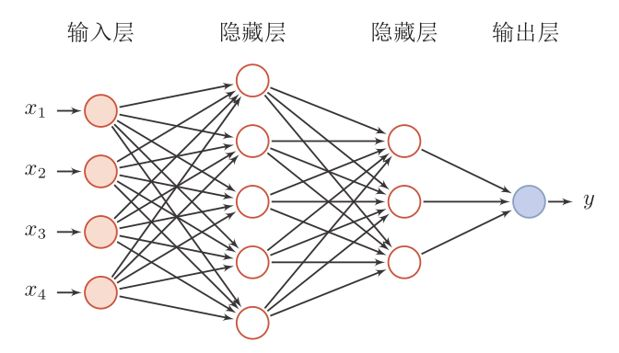
\includegraphics[width=0.7\textwidth]{ANN}
    \caption[ANN]{具有两个隐藏层的神经网络}
    \label{ANN}
\end{figure}
\newpage
其中一种最基本的人工神经网络就是单层前馈神经网络,其只有一个输出层,输出层上节点的值作为输出值,通过输入值乘以权重直接得到。如果取出其中一个神经元进行具体分析的话,其从输入映射到输出的变换关系如公式~\ref{eq:ns}和公式~\ref{eq:ns2}
\begin{equation}
    \label{eq:ns}
        S_{j}=\sum ^{n}_{i=1}w_{ji}x_{i}-\theta _{j}
\end{equation}
\begin{equation}
    \label{eq:ns2}
    y_{i}=f\left( s_{i}\right) =\begin{cases}1,x_{i}=0\\
    0,x_{i} <0\end{cases}
\end{equation}
上式中,x是输入的特征向量,w是x到y的连接权值,输出量y是按照不同特征的分类而产生的结果。

权值越大表示输入信号对神经元影响越大。而如果权值是负值,那意味着抑制输入信号。我们可以得知,如果权不同,那么元的计算情况也不同。那么通过调整权值就可以获得相同输入情况下我们不同需要输出的值。但是这些ANN是由成百上千的人工神经元组成的,人工计算这些权值只有理论实现的可能。我们必须使用一定的算法去简化其工作难度。而这种采用一定算法自动化调整权重的过程称为训练或者学习。

人工神经网络的目标是通过找到最小化训练数据误差的参数来找到最佳函数近似值。通过对处理后的数据集训练来学习这些参数。对于每个预测y,与真实的结果相比,测量误差。

为了减小这些误差,我们可以采取如下策略:

策略1:随机寻找,这种方法其实并不特别实用,这是最直接粗暴的方法,就是我们尽量多地去穷尽参数,然后从里面选一个能够让loss最小的参数组,来作为最后的W。

策略2:随机局部搜索,就是我们可以在建立在参数W基础上,随机地搜索一下周围的参数,去计算观察一下是否有比现在更好的W,然后用这个新的W替换之前的W,然后不断迭代。

策略3:使用梯度下降算法,也就是找到最陡的方向下山,每走一小步,就去寻找当前位置最陡的下山方向,继续前进一小步。而反向传播是用来计算上述中梯度的快速算法。
\section{递归神经网络}\label{sec:background}
有两种人工神经网络都被称之为递归神经网络(RNN)\cite{DBLP:journals/corr/KannanKRKTMCLGY16}。其一是时间递归神经网络(recurrent neural network),其二是结构递归神经网络(recursive neural network),这两者都简称为RNN。神经元之间会连接构成有向图就是时间递归神经网络,而利用相似的神经网络结构不断递归从而构造更为复杂的深度网络的就是结构递归神经网络会。两者训练的算法虽然不同,但是本质则师出同门。本论文的聊天机器人模型主要运用的为时间递归神经网络,所以下文涉及到的RNN全部都为时间递归神经网络。

传统的人工神经网络叫做FNN(Feed-Forward Neural Networks),也就是前馈神经网络,有关传统神经网络的介绍上文已经提过,RNN是在此基础上引入了定向循环,也就是已神经元为节点组成的图中存在有向的环,这种神经网络可以表达某些前后关联关系,事实上,这种环形信息传播的结构也是真正的生物神经元之间传递的方式,RNN也是人工神经网络向真实生物神经网络靠近的一个进步\cite{Goodfellow-et-al-2016}。一个典型的RNN如图~\ref{RNN}所示。
\begin{figure}[!htbp]
    \centering
    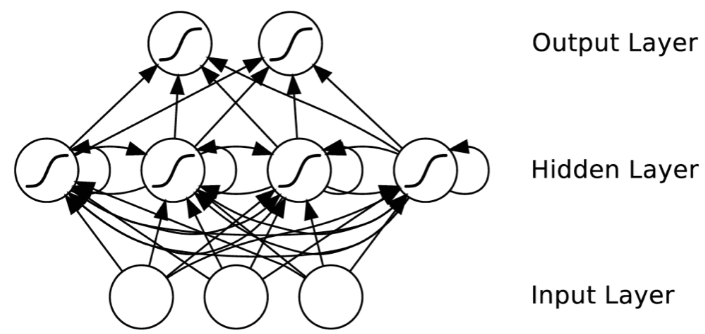
\includegraphics[width=0.70\textwidth]{RNN}
    \caption[RNN]{递归神经网络}
    \label{RNN}
\end{figure}

图中隐藏层中的节点之间构成了全连接,也就是在一个隐藏层中,某一个节点的输出可以作为另一个隐藏层的节点的输入,甚至它同时可以是自己所在隐藏层的输入,这种结构可以抽象成图~\ref{RNN1}。
\begin{figure}[!htbp]
    \centering
    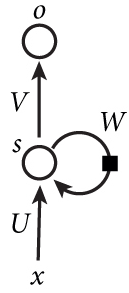
\includegraphics[width=0.1\textwidth]{RNN1}
    \caption[RNN1]{RNN抽象结构}
    \label{RNN1}
\end{figure}

在RNN中,所有隐藏层中的参数由所有时间步骤共享。因为上述这个原理,从而每一个梯度取决于先前的时间步长。为了训练RNN,使用了一种称为反向传播的算法(BPTT)。

当使用反向传播算法时,学习的长期依赖性存在困难\cite{279181}。由于反向传播使用链规则计算梯度,因此有许多小数相乘,导致远离最终层的层的梯度变得极小或消失。有一些方法可以避免这个问题,例如使用门控递归神经网络,例如,长期短期记忆(LSTM)\cite{Graves2012Long}或更近期的门控循环单元(GRU)\cite{DBLP:journals/corr/ChoMGBSB14}。 

特别讲解一下LSTM,因为LSTM正是本文使用的人工神经网络模型,其是一种特别的RNN,也是RNN能应用成功的关键。RNN存在一个长序列依赖(Long-Term Dependencies)的问题:下一个词的出现的概率和很久之前出现的词有关,但因为计算量的限制,依赖的长度就必须得到一定的限制。所以LSTM被专门的设计出来来很好地解决这个问题。

LSTM最初是由Hochreiter和Schmidhuber引入的\cite{Graves2012Long},是一种旨在更好地处理长期依赖性的RNN。与常规RNN的不同之隐藏状态的计算方法。LSTM具有内部单元状态,并且能够添加或从状态中删除信息。添加或删除的内容由称为门的结构调节。通常,有三个门称为输入门,遗忘门和输出门。输入门和遗忘门决定新输入的数量的多少添加进新状态以及从旧的单元状态丢掉的数据来控制每一个单元的状态。同时输出门根据单元状态来决定输出的数据。这些门允许LSTM处理长期依赖性,LSTM通过学习门的参数来最终学会如何对输入的语言进行分析回复。
\section{序列到序列的模型}\label{sec:background}
一种使用递归神经网络的模型是seq2seq模型,有时称为encoder-decoder模型\cite{DBLP:journals/corr/ChoMGBSB14}。该模型用于学习从序列到序列的映射。这个基本思想可以用于许多高级任务。两个例子是机器翻译\cite{Sutskever2014Sequence}和对话模型\cite{DBLP:journals/corr/VinyalsL15}。在机器翻译中,目标是将一种语言的单词序列映射到另一种语言的相应单词序列。在对话模型中,目标是从输入句子转换为对应的回复句子。

序列到序列模型存在许多变体,但基本结构由两个RNN组成。将输入编码为矢量表示,捕获输入序列的含义和重要信息。然后另一个RNN将此向量作为输入并使用它来产生输出序列。该过程用图~\ref{seq2seq}中的展开的RNN描述。
\begin{figure}[!htbp]
    \centering
    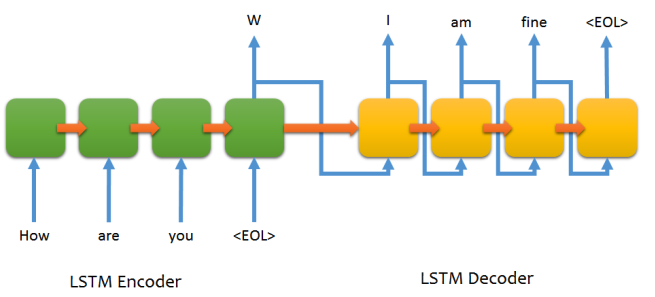
\includegraphics[width=0.8\textwidth]{seq2seq}
    \caption[seq2seq]{序列到序列的模型(LSTM为例)}
    \label{seq2seq}
\end{figure}


在该图中,每个框是RNN小区,例如LSTM或GRU。该编码器按词读取输入,直到获得
代表着结尾的特殊标记,在图中,此标记为<EOL>。基于在编码器生成的上下文中,解码器生成输出句子,一个词一个词,直到它生成一个结束字符。在每一个时序,先前生成的语句被反馈到网络中重新作为输入。

在每个时序步骤中,解码器产生可能推断的词汇概率列表。这些概率用于计算生成序列与现有序列匹配的概率。用贪心搜索的话,就是在每个时序中选择概率最高的词语,并将其反馈到网络中以生成下一个词语\cite{Sutskever2014Sequence}。当然我们也可以选择了概率最大的前k个。这个k值也叫做集束宽度(Beam Width),而不是考虑每个时序中最可能的标记。

为了计算给输入序列到输出序列的概率,我们使用条件概率p(y1,y2,...,ym | x1,x2,...,xn)[28],其中xi是输入标记和yi是输出标记。在图~\ref{seq2seq}的例子中,这将是p(i,am,fine | How,are,you)。这个概率可以改写成下方公式~\ref{eq:ns3}。
\begin{equation}
    \label{eq:ns3}
    P( y_{1},\ldots ,y_{m}\mid x_{1},\ldots ,x_{n}) = \prod ^{m}_{i=1}p( y_{i}\mid x_{1},\ldots ,x_{n},y_{1},\ldots ,y_{i-1} )   
\end{equation}

因此,我们计算在所有当前时序下的每个词语概率的乘积,从一组可能的序列中选择输出可能性最高,也就是最可能匹配的序列。
\section{记忆网络}\label{sec:background}
神经网络善于学习和模拟,但难以记住它们。seq2seq中的记忆依靠RNNCell或者LSTMCell实现,但是RNN和LSTM的记忆能力不能令人满意,记忆十几个时间步长的信息也就达到了极限。因此当句子长度达到一定程度或者先验知识需要被添加的时候,seq2seq就不能满足当前对话模型的需求。对此的解决方案是使用内存组件来存储和检索特定数据。使用长期存储组件来存储信息的存储器,并将其与用于推测的组件结合使用以进行预测,模型将学习如何一起使用这些组件。由Sukhbaatar等人介绍的端到端存储网络\cite{Perez2016Gated},是一种端到端的可训练的内存网络。比起人工增加RNN隐藏层大小,我们更愿意任意增加模型的所可以储存记忆量,这样我对模型本身并不需要作出多大的改变。基本上,我们可以把独立存储器作为一种人工神经网络。模型可以从中按照需要进行读写,以此来强化人工神经网络性能。拿计算机系统当作类比的话,CPU即神经网络,RAM就是这种新的外部存储器。
\section{语料表示方法}\label{sec:background}
聊天机器人的训练数据是来自于大量的自然语言的对话,并且许多机器学习算法要求输入是定长的特征向量\cite{Le2014Distributed},所以必须得对语料库进行处理。

有很多不同的方式来表示一个单词。一种简单的方法是使用One-Hot编码\cite{马广才2011状态机编码的低功耗设计}。每个单词由多个0和单个1的向量表示,这种方法确保词汇表中的每个单词都由唯一的向量表示。但是由于词汇量很大,这些向量变得庞大且数据非常稀疏,而且这种编码不提供有关单词之间关系的任何有用信息。

为了限制向量空间的维数,我们可以使用一种称为嵌入的技术。单词嵌入是将单词映射到高维向量的函数\cite{Bengio2006Neural}。这种函数通常是可查找的,并且是一个矩阵,在词汇表中,每个单词都是一行记录。每个单词的随机向量用来初始化矩阵,当前存在许多不同的嵌入方法,例如Mikolov等人的word2vec模型。\cite{DBLP:journals/corr/MikolovSCCD13}。该模型不仅限制了维度,还可以显示出单词之间的关系。例如,土豆和马铃薯,会得到十分接近的向量,因为它们具有相同的含义,为解决一词多义提供了巨大的帮助。
\end{cuzchapter}
\begin{cuzchapter}{聊天机器人实践}{chap:introduction}
本章首先介绍本文实践的聊天机器人的任务目标,之后是对用于训练和评估的数据集进行讨论并进行收集爬取工作。接下来描述了模型的实现细节,训练方式以及降低损失率的方法。最后将介绍如何将训练有素的模型用于社交软件中并设计相应的安卓插件。
\section{问题描述}\label{sec:background}
在本论文中,实现一个序列到序列的对话模型的创建,完成一个实现日常闲聊任务的聊天机器人。利用QQ和用户进行正常的闲聊对话,能够进行一定的问答,心理疏导,娱乐等功能。

为了实现其目标,聊天机器人必须能够正确处理和解释自然语言的输入。基于此输入,机器人必须快速分析,查询记忆网络以检索信息,找出合适的回答,向用户显示结果。并跟着用户的对话思路,调整对话技巧,让用户感受到与真人聊天一般的感觉。
\section{语料库的收集}\label{sec:background}
从真实对话中收集的数据通常包含各种噪音如拼写错误,错误信息,解释错误和
所以这使得训练更加困难。在更大或更开放的适用面上也变得更难以学习。对话涉及的范围,可能答案的数量就越多。所以本文首先采用了公开的语料库,腾讯公司开源的中文语料库涉及面广,用词准确,非常适合作为聊天机器人训练的基础语料,无需其他的繁琐的操作,可以直接使用。

但对于普通的生产科研环境下,开源语料库的内容涉及面过于宽泛,过大,训练时间复杂度也相应提高,普通设备也难以支撑此高强度的训练工作,于是,还是需要寻找相关的语料库去替代。但是一般网上的其他语料库基本都是杂乱无章的,并没有可用的对话语料,所以我们可以另辟蹊径,获取海量高可用价值的语料库。高质量的电影或电视剧的字幕文件包含着大量的可用对话数据,尤其是对话多的影视作品。为了获得这些高质量的自然语言的对话素材,本文打算爬取字幕库网站www.zimuku.net。

首先我们先得从互联网上爬取字幕,如附录代码段~\ref{code:catch}和~\ref{code:catchm}。运行完简单的爬虫程序可以获得大量的字幕压缩文件。

但是下载的字幕压缩格式五花八门,因为数据总量比较多,所以必须得做一点筛选分类,不然会影响后续的工作。其中的问题例如扩展名种类过多、文件名重名是否错误覆盖、文件名带特殊字符,于是得开始一系列处理。如代码段~\ref{code:mv_zip}。把其中压缩文件可能有的扩展名*.rar、*.RAR、*.zip、*.ZIP等,把他们按不同的后缀分别放到不同的目录下去。
\begin{lstlisting}[
    language=python,
    label=code:mv_zip,
    caption=压缩格式分类
]
import glob
import os
import fnmatch
import shutil
import sys

def iterfindfiles(path, fnexp):
    for root, dirs, files in os.walk(path):
        for filename in fnmatch.filter(files, fnexp):
            yield os.path.join(root, filename)

i=0
for filename in iterfindfiles(r"./input/", "*.zip"):
    i=i+1
    newfilename = "zip/" + str(i) + "_" + os.path.basename(filename)
    print filename + " <===> " + newfilename
    shutil.move(filename, newfilename)
\end{lstlisting}

再把各类压缩文件分类统一之后,就可以开始进行解压工作,为了解决解压后文件重名可能导致的覆盖问题,本文使用如下脚本代码段~\ref{code:unzip}以实现解压安全自动化:
\begin{lstlisting}[
    language=python,
    label=code:unzip,
    caption=批量解压
]
class SubtitleCrawlerPipeline(object):
    def process_item(self, item, spider):
        url = item['url']
        file_name = url.replace('/','_').replace(':','_')
        fp = open('result/'+file_name, 'w')
        fp.write(item['body'])
        fp.close()
        return item
\end{lstlisting}

解压后发现字幕文件的后缀名有很多种,其中包括idx、str、vtt、srt、lrc、ass、ssa、sup,但是整体体量大小上说srt、ass、ssa占绝对优势,因此为了减少不必要的麻烦,其他格式全部放弃,只保留这三种,并且把不同扩展名的文件分类保存到不同的目录下,方法同压缩文件格式的处理相同,具体见附录代码段~\ref{code:mv_ass},~\ref{code:mv_Irc},~\ref{code:mv_smi},~\ref{code:mv_srt},~\ref{code:mv_ssa},~\ref{code:mv_str},~\ref{code:mv_sup},~\ref{code:mv_vtt}。

在进行后缀名分类归纳的时候,为了避免重名的问题,建立了很多不同的文件夹,但是进一步后缀名整理之后,空目录会大量产生,所以必须进行一个自动清理空目录的过程,见代码段~\ref{code:clean}。
\begin{lstlisting}[
    language=python,
    label=code:clean,
    caption=清理目录
]
import glob
import os
import fnmatch
import shutil
import sys

def iterfindfiles(path, fnexp):
    for root, dirs, files in os.walk(path):
        if 0 == len(files) and len(dirs) == 0:
            print root
            os.rmdir(root)

iterfindfiles(r"./input/", "")
\end{lstlisting}

在字幕文件的处理过程中,有许多不需要的文件,比如html、txt、doc、docx,这些不是本文所需要的,因此直接删掉,见代码段~\ref{code:delete}。
\begin{lstlisting}[
    language=python,
    label=code:delete,
    caption=删除非字幕文件
]
import glob
import os
import fnmatch
import shutil
import sys

def iterfindfiles(path, fnexp):
    for root, dirs, files in os.walk(path):
        for filename in fnmatch.filter(files, fnexp):
            yield os.path.join(root, filename)

for suffix in ("*.mp4", "*.txt", "*.JPG", "*.htm", "*.doc", "*.docx", "*.nfo", "*.sub", "*.idx"):
    for filename in iterfindfiles(r"./input/", suffix):
        print filename
        os.remove(filename)
\end{lstlisting}

进行上述一系列操作之后,就可以开始对字幕文件的处理了。因为字幕文件没有什么规范标准,于是各种编码齐聚一堂,utf-8、utf-16、gbk、unicode、iso8859等编码方式无所不有,所以统一到一种编码会带来极大的方便,于是统一到utf-8,见附录代码段~\ref{code:encode}。

鉴于本文的目标和问题的要求,旨在解决中文聊天机器人的制作,所以删去其中其他语言的对话内容,进行语言的筛选,见附录代码段~\ref{code:extract}。

经过上面复杂繁琐的处理,本文就已经获取可用的语料库,只是里面不是对话的内容必须得进行更近一步的处理,包括:过滤特殊字符、去除特殊的关键词、去除字幕样式flag、html标签、特殊字符、转义字符、剧集信息等等各式各样的标志,具体见附录代码段~\ref{code:filter}。中文高质量语料库就此获得。

除了开源大型语料库和上述的爬取字幕的处理后的语料,最后本文还选取了个人的聊天记录作为语料。这类的语料库,语言风格纯净,更能反映个人的风格个性,作为个性化的训练模型,最终个人的聊天机器人,选取个人的聊天记录作为语料库进行训练,方便快捷,能够更好塑造风格一致的聊天机器人。
\section{评估方法}\label{sec:background}
聊天机器人的目标是完成个人闲聊交谈功能。通过测量系统来评估其性能,根据到目前为止的谈话,预测回复的能力。例如,考虑由话语{u1,b1,u2,b2,...,un,bn}组成的对话,其中ui是用户话语,bi是话语权。 此对话将分为c1 = {u1},r1 = {b1},c2 = {u1,b1,u2},r2 = {b2}等等,其中ci是上下文,ri是给定的正确响应上下文。不同的权值会影响到不同回复正确性对整体的影响,当然针对闲聊来说,寒暄所占的权值就比较低,有质量的对话占的权值就会更高。

如果只考虑数据集中对话来判断预测的回复是否正确,那评估标准会是想当的严格。例如,如果正确的答案是“谢谢”,那么说“谢了”是不正确的。 然而数据集中没有这种模糊性。最终成果的检测还是必须得人类自己来判断。

每次回复都会影响整次会话准确度,如果出现一些答非所问,必然会降低用户的体验感。响应准确度衡量机器人能够预测正确响应的响应百分比。会话准确度计算为正确预测回复的次数。最终将以正确相应的次数表示的精准度来判断模型是否足够优秀。
\section{模型构建方法}\label{sec:background}
本文聊天机器人的目标是根据上下文预测出正确的回复。因此,在训练期间,通过考察条件概率p(response|context),就是在上下文的条件下,得出的语句的概率。而训练模型要选择尽可能高的概率的语句作为回复。

上下文和响应都可以是一系列单词,所做的即在给定先前看到的标记序列的情况下预测最可能的标记序列,即最大化p(r1,...,rn | c1,...,cm)。鉴于模型目标的这种表述,使用的模型是序列到序列学习。这是一个众所周知的模型,存在于许多变体中,并已成功用于几种自然语言任务。

每个单独的预测都有一个关联的分数(或概率),我们只对最大分数(或最大概率)的输出序列感兴趣。一种流行的近似方法是使用贪心搜索,即在每个阶段采用得分最高的项。虽然这种方法通常是有效的,但显然不是最佳的。实际上,用集束搜索作为近似搜索通常比用贪心搜索要好得多。
\section{词向量生成方法}\label{sec:background}
收集来的语料库,并不能直接让模型去学习,必须通过分词把句子分割成一个个的词语,再把词语转化为词向量。为了让机器能理解自然语言,NLP(自然语言处理)是第一步。

jieba是目前最好Python中文分词组件之一。这种第三方分词库拥有三种分词模式,精确地将句子切开从而进行文本分析这是最基本的功能。通过基于前缀词典就可以实现词图扫描,并把生成句子中中文字词所有可能成词的情况统一收集分析,把他们构成一个有向无环图。

分词之后,就必须提到词向量,这是是将深度学习应用到NLP的大门,而如今使用最广泛训练工具同时也是本文使用的word2vec,其简单高效。我们采用distributed representation,中文释义是分布式表达的方式,将词转化为词向量。具体代码见附录代码段~\ref{code:word2rec}

\section{实施}\label{sec:background}
本文使用开源机器学习实现库Tensorflow。序列到序列模型基于Tensorflow中的tf.contrib.seq2seq模块。

编码器和解码器都包含动态RNN,意思是他们对序列长度没有限制。Tensorflow中的常规RNN是在内部创建了一个具有固定长度的RNN的,这限制了输入的最大允许长度。动态RNN实现允许不同大小的输入。编码器RNN和解码器RNN都使用LSTM。LSTM实现在tf.contrib.rnn模块中定义,并基于Hochreiter和Schmidhuber的论文\cite{Graves2012Long}。每个单元可以具有多个单位。这是指单元隐藏状态的大小,决定了神经网络的学习能力。使用更多单位可以记住更的训练数据,但是训练需要更长时间并且存在过拟合的风险。通常更多单位通常不会给出明显更好或更差的结果,但一般都会大大放慢了训练速度。

对话数据上下文配对。这些字符串被标记,每个单词被分配一个索引。这些序列表就构成了模型的输入和输出。然后,该模型将这些序列表转化成向量表示,这就是模型训练的任务。
\subsection{接口和参数}\label{sec:background}
下面本文就会集中于使用tensorflow,其拥有众多强大api给我们使用,想要利用好它,重要接口及其参数就必须了解清楚,其如下代码段的~\ref{code:seq2seq}。
\begin{lstlisting}[
    language=python,
    label=code:seq2seq,
    caption=seq2seq接口
]
embedding_attention_seq2seq(
    encoder_inputs,
    decoder_inputs,
    cell,
    num_encoder_symbols,
    num_decoder_symbols,
    embedding_size,
    num_heads=1,
    output_projection=None,
    feed_previous=False,
    dtype=None,
    scope=None,
    initial_state_attention=False
)
\end{lstlisting}

为了说明这个接口的功能,先来看一下它所涉及到的模型结构,如图~\ref{seq2seq2}所示
\begin{figure}[!htbp]
    \centering
    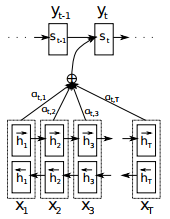
\includegraphics[width=0.3\textwidth]{seq2seq2}
    \caption[seq2seq2]{seq2seq结构}
    \label{seq2seq2}
\end{figure}

参数encoder\_inputs为list容器,list中每一项是为一个Tensor,这个Tensor的shape是[batch\_size],Tensor中的每项都是一个整型,类似于下代码段~\ref{code:array}。
\begin{lstlisting}[
    language=python,
    label=code:array,
    caption=示例
]
[array([0, 0, 0, 0], dtype=int32), 
array([0, 0, 0, 0], dtype=int32), 
array([5, 0, 2, 5], dtype=int32), 
array([0, 7, 0, 6], dtype=int32), 
array([0, 0, 1, 6], dtype=int32)]
\end{lstlisting}
其中的5个array,表示一句话的长度是5个词

其中每个array里数的个数就是batch的大小,也就是一共4个样本。那么从中就可以看出第一个样本是[[0],[0],[5],[0],[0]],第二个样本是[[0],[0],[0],[7],[0]],这里的数字也就是所谓的ID。同理,参数decoder\_inputs也是和encoder\_inputs一样结构。

参数cell是tf.nn.rnn\_cell.RNNCell类型的循环神经网络单元。

num\_decoder\_symbols表示decoder\_inputs中整数词id的数目。

embedding\_size表示在模型在做word embedding时转化向量的维度数,需要和RNNCell的size大小相等。

num\_heads表示在attention\_states中的抽头数量。

output\_projection是一个(W, B)结构的tuple,W是shape为[output\_size x num\_decoder\_symbols]的weight矩阵,B是shape为[num\_decoder\_symbols]的偏置向量,那么每个RNN单元的输出,经过WX+B就可以映射成num\_decoder\_symbols维的向量,这个向量里的值表示的是任意一个decoder\_symbol的可能性,也就是softmax。

feed\_previous表示decoder\_inputs是作为输入,我们直接用训练使用的语料库把他填入,还是用前一个RNN单元的输出出来的,如果feed\_previous为True,那么使用先前cell的输出,并经过数学映射成默认是tf.float32的RNN状态数据的类型。

scope是子图的命名,默认是“embedding\_attention\_seq2seq。initial\_state\_attention默认全都为0,就是全否,就是attentions全未初始化。

一个(outputs, state)结构的tuple是它的返回值,其中outputs是一个句子长度(词数,与上面encoder\_inputs的list长度一样)的list,这里所谓的list中每项是一个二维的tf.float32类型的Tensor,样本数是第一维度,有多少个样本就多少个组Tensor,每个Tensor长度是embedding\_size。
\subsection{模型构建}\label{sec:background}
那么我们如何使用上节所说的参数来构建seq2seq的模型呢。

我们以奇数序列为例来构造样本从而训练出可预测奇数数列的模型,比如两个样本分别是[[1,3,5],[7,9,11]]以及[[3,5,7],[9,11,13]],把他们填入接口中就是:train\_set = [[[1, 3, 5], [7, 9, 11]], [[3, 5, 7], [9, 11, 13]]]。
那么我们的第一个样本的encoder\_input就是:
\begin{lstlisting}[
    language=python,
    label=,
    caption=
]
encoder_input_0 = [PAD_ID] * (input_seq_len - len(train_set[0][0])) + train_set[0][0]
\end{lstlisting}

第二个样本的encoder\_input就是:
\begin{lstlisting}[
    language=python,
    label=,
    caption=
]
encoder_input_1 = [PAD_ID] * (input_seq_len - len(train_set[1][0])) + train_set[1][0]
\end{lstlisting}
=需要用一个GO\_ID来作为decoder\_input的起始,再输入样本序列,最后填充PAD\_ID,即
\begin{lstlisting}[
    language=python,
    label=,
    caption=
]
GO_ID = 1
decoder_input_0 = [GO_ID] + train_set[0][1] 
    + [PAD_ID] * (output_seq_len - len(train_set[0][1]) - 1)
decoder_input_1 = [GO_ID] + train_set[1][1] 
    + [PAD_ID] * (output_seq_len - len(train_set[1][1]) - 1)
\end{lstlisting}

把输入转成上面讲到的embedding\_attention\_seq2seq输入参数encoder\_inputs和decoder\_inputs的格式,我们进行如下转换即可:
\begin{lstlisting}[
    language=python,
    label=,
    caption=
]
encoder_inputs = []
decoder_inputs = []
for length_idx in xrange(input_seq_len):
    encoder_inputs.append(np.array([encoder_input_0[length_idx], 
                          encoder_input_1[length_idx]], dtype=np.int32))
for length_idx in xrange(output_seq_len):
    decoder_inputs.append(np.array([decoder_input_0[length_idx], 
                          decoder_input_1[length_idx]], dtype=np.int32))
\end{lstlisting}

把参数的输入搞定之后,我们创建encoder\_inputs和decodr\_inputs的placeholder(占位符)。
\begin{lstlisting}[
    language=python,
    label=,
    caption=
]
encoder_inputs = []
decoder_inputs = []
target_weights = []
for i in range(input_seq_len):
    encoder_inputs.append(tf.placeholder(tf.int32, shape=[None], name="encoder{0}".format(i)))
for i in range(output_seq_len + 1):
    decoder_inputs.append(tf.placeholder(tf.int32, shape=[None], name="decoder{0}".format(i)))
for i in range(output_seq_len):
    target_weights.append(tf.placeholder(tf.float32, shape=[None], name="weight{0}".format(i)))
\end{lstlisting}

然后接着创建LSTM单位,设置大小。
\begin{lstlisting}[
    language=python,
    label=,
    caption=
]
cell = tf.contrib.rnn.BasicLSTMCell(size)
\end{lstlisting}

把参数传给embedding\_attention\_seq2seq获取输出outputs。
\begin{lstlisting}[
    language=python,
    label=,
    caption=
]
outputs, _ = seq2seq.embedding_attention_seq2seq(
    encoder_inputs,
    decoder_inputs[:output_seq_len],
    cell,
    num_encoder_symbols=num_encoder_symbols,
    num_decoder_symbols=num_decoder_symbols,
    embedding_size=size,
    output_projection=None,
    feed_previous=feed_previous,
    dtype=tf.float32)
\end{lstlisting}

来构造运行时的session,并填入样本数据。
\begin{lstlisting}[
    language=python,
    label=,
    caption=
]
for l in range(input_seq_len):
input_feed[encoder_inputs[l].name] = sample_encoder_inputs[l]
for l in range(output_seq_len):
input_feed[decoder_inputs[l].name] = sample_decoder_inputs[l]
input_feed[target_weights[l].name] = sample_target_weights[l]
input_feed[decoder_inputs[output_seq_len].name] = np.zeros([len(sample_decoder_inputs[0])], dtype=np.int32)
\end{lstlisting}

这里的outputs实际上应该对应seq2seq的输出,也就是下图~\ref{output}中的W、X、Y、Z、EOS,也就是decoder\_inputs[],也就是我们样本里的[7,9,11]和[9,11,13]
\begin{figure}[!htbp]
    \centering
    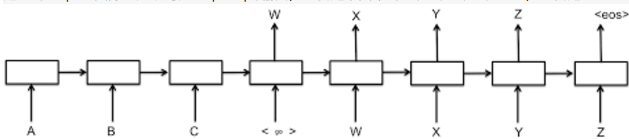
\includegraphics[width=0.8\textwidth]{output}
    \caption[output]{}
    \label{output}
\end{figure}
\subsection{训练}\label{sec:background}
使用tf.contrib.seq2seq模块中定义的Tensorflow函数sequence\_loss对序列表使用加权交叉熵损失对模型进行训练。如Kingma和Ba\cite{DBLP:journals/corr/Adam}所述,使用Adam优化器可以将损失最小化。利用一阶矩估计以及二阶矩估计,学习率保持不动,所以不管经过多少轮的迭代,学习率都在一个范围之内,这样参数就可以很平稳的变化。

模型经过了多轮的训练,遍历整个语料库。每轮训练后,验证模型的损失率和精度。当精度不再提高时,训练终止。

那下面就是这个损失率的事情了,loss函数的参数如下:
\begin{lstlisting}[
    language=python,
    label=,
    caption=
]
sequence_loss(
    logits,
    targets,
    weights,
    average_across_timesteps=True,
    average_across_batch=True,
    softmax_loss_function=None,
    name=None
)
\end{lstlisting}

这个函数的原理如公式~\ref{eq:ns4}:
\begin{equation}
    \label{eq:ns4}
    loss=-\dfrac {1}{N}\sum ^{N}_{i=1}\ln P_{t\arg et}  
\end{equation}

其中logits是一个由多个2D的shape为[batch * num\_decoder\_symbols]的Tensor组成的list,batch就是2,相对的num\_decoder\_symbols的batch就是16,整个list的Tensor的个数为output\_seq\_len,所以我们刚才得到的outputs刚好符合。其中targets是一个和logits一样长度(output\_seq\_len)的list,list里每一项是一个整数组成的1D的Tensor,每个Tensor的shape是[batch],数据类型是tf.int32,这刚好和我们的decoder\_inputs[]也就是刚才说的W、X、Y、Z、EOS结构一样。其中weights是和targets结构相符合,tf.float32为数据类型。

计算加权交叉熵损失的就是如下这个函数:
\begin{lstlisting}[
    language=python,
    label=,
    caption=
]
target_weights = []
    target_weights.append(tf.placeholder(tf.float32, shape=[None], 
                          name="weight{0}".format(i)))
)
\end{lstlisting}
计算得出的损失值就是:
\begin{lstlisting}[
    language=python,
    label=,
    caption=
]
targets = [decoder_inputs[i + 1] for i in xrange(len(decoder_inputs) - 1)]
loss = seq2seq.sequence_loss(outputs, targets, target_weights)
)
\end{lstlisting}

定义好loss之后,就开始真正的训练,去降低loss,运用梯度下降来更新参数。本文使用Tensorflow提供的梯度下降优化器GradientDescentOptimizer。
于是乎,计算损失率梯度并更新参数的方法如下:
\begin{lstlisting}[
    language=python,
    label=,
    caption=
]
learning_rate = 0.1
opt = tf.train.GradientDescentOptimizer(learning_rate)
update = opt.apply_gradients(opt.compute_gradients(loss))
\end{lstlisting}

最后我们通过main函数不断的循环迭代梯度下降,经过不断的循环,最终符合要求的模型就训练好了。
\begin{lstlisting}[
    language=python,
    label=,
    caption=
]
def get_model():
      ...
saver = tf.train.Saver(tf.global_variables())
      return ..., saver
\end{lstlisting}

接下来,我们如果去做预测,那么理论上不能有decoder\_inputs的输入了,执行decoder\_inputs就必须得需要前面一个时序的输出,在这个时候,神兵降临embedding\_attention\_seq2seq的feed\_previou就有了存在的意义和价值,这个参数若为True则decoder里每一步输入都用前一步的输出来填充,如下图~\ref{previous}。
\begin{figure}[!htbp]
    \centering
    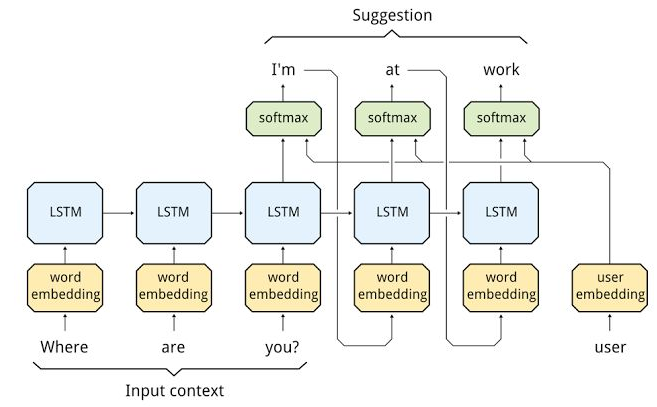
\includegraphics[width=1\textwidth]{previous}
    \caption[previous]{}
    \label{previous}
\end{figure}

所以,我们的get\_model需要传递不同参数,来区分不同的阶段,也就是训练和预测,那么feed\_previous就需要不同的配置,另外,考虑到预测时main函数也是不同的,索性我们分开两个函数来分别做train和predict,完整代码见附录代码段~\ref{code:train}以及附录代码段~\ref{code:predict}。
\subsection{安卓插件的制作}\label{sec:background}
为了应用中文聊天机器人的模型以及测试效果,本文使用模型来创建一个基于xposed的安卓插件,该应用程序能hook QQ中的聊天信息,并将消息发送至服务器上部署的模型,服务器上的模型解释用户输入并生成回复。给定输入后,模型通过一个单词一个单词地进行预测,然后将用户输入和模型回复添加到上下文集中,以跟踪以往所说内容。出于实用目的,上下文的大小是有限的,聊天机器人会开始“忘记”很久以前说过的话。这个限制可以调整,以使得系统有一个更长的或更短的内存。在本文的实例中,使用的限制等于训练数据中最长的对话。随着对话的进行,模型要做的就是对给定的上下文和下一个用户输入进行预测,以此下去。

为了与QQ的实时消息关联,本文采用了Xposed框架(Xposed Framework)。其是一套开源的、在安卓ROOT权限下的一种服务框架,在不修改APK源码的情况下,直接安卓应用的运行(修改系统),这是它最重要的功能,基于它可以制作出许多功能强大的插件。

下面通过xposed强大的功能,hook到我想要获取的方法函数,获取我想要的域,见附录代码段~\ref{code:get}。调用上述函数完成如下代码段~\ref{code:getmsg}的信息获取。
\begin{lstlisting}[
    language=java,
    label=code:getmsg,
    caption=获取信息
]
final String frienduin = getObjectField(param.args[1], "frienduin").toString();
final String selfuin = getObjectField(param.args[1], "selfuin").toString();
final int istroop = (int) getObjectField(param.args[1], "istroop");
final String senderuin = getObjectField(param.args[1], "senderuin").toString();
final String msg = getObjectField(param.args[1], "msg").toString();
boolean isread = (boolean) getObjectField(param.args[1], "isread");
\end{lstlisting}

经过上述操作后,已经获取到了聊天消息,下面就要着手准备发送数据给服务器端的模型,让模型去分析处理了。本文采用socket,进行通信编程,封装的函数见附录代码段~\ref{code:socket} 。

我们利用Xposed在QQ的设置中嵌入一个新的设置页面,如图~\ref{qqrobot}所示。并把该页面注入到QQ设置页面中去见附录代码段~\ref{code:inject}。
\begin{figure}[!htbp]
    \centering
    
\includegraphics[width=0.5\textwidth]{qqrobot}
    \caption[qqrobot]{插件设置主页}
    \label{qqrobot}
\end{figure}

由此消息的交互就基本完成,完整代码见附录代码~\ref{code:commnucation}。
\end{cuzchapter}
\begin{cuzchapter}{结果及比较}{chap:introduction}

经过了漫长复杂的学习实践过程,最后对成果进行分析。如果是分类问题,那么100\%准确的就是最佳分数;如果是回归问题,0误差就是最佳分数。这些分数其实都不可能完全达到上限或下限。所有的预测建模问题都存在预测误差。那么误差出现在哪里呢。误差来源范围包括:1、不完整的数据样本;2、数据中的干扰信息;3、建模算法的随机性。

\section{模型性能分析}\label{sec:background}
我们的序列到序列模型的准确性与几个基线模型进行了比较,其他基线模型取自Bordes等人\cite{DBLP:journals/corr/BordesW16},并通过相同语料库训练得出。基线模型包括基于规则的模型,两个经典信息检索模型和两个基于网络的模型。

序列到序列模型在所有任务上都优于传统的信息检索模型。与监督嵌入模型相比,它也获得相同或更好的结果。我们的模型的准确性类似于没有匹配类型功能的记忆网络。通过匹配类型功能,记忆网络可以在大多数任务中获得最佳结果,匹配类型功能似乎可以改善结果,特别是在训练语料库之外测试。 

我们模型的准确性与上述模型通过100条对话进行人工测试,进行对比,结果显示在表格~\ref{tab:sample}中,都以百分比的形式表示,如果得到正确有意义的回复便是1,否则即为0。如果使用在训练时的语料库中的词语事,我们的序列到序列模型可以达到100%准确性,这意味着每个响应都被正确预测。当使用在不在训练语料库中的词语进行测试时,每个响应的准确度大幅度下降。在进行这类测试的时候,模型完全无法从已经训练成型的多维空间中找到合适的词向量,基本都是以预设的报错回复相应,即使找到多维空间中的词向量,也可能无法构成通顺有意义的语句。而设计到个性化的问答,感情的抒发,模型也没法完整作出良好的回复,毕竟每个人的个性不尽相同,不能都和空间中的向量完全匹配。

\begin{table}[]
    \centering
    \caption{基线模型结果比较表}
    \label{tab:sample}
    \begin{tabular}{|c|c|c|c|c|c|}
    \hline
     & 日常闲聊 & 信息询问 & 情感表达 & 个性化问答 & oov \\ \hline
    基于规则 & 100 & 100 & 34 & 24 & 0 \\ \hline
    最邻近规则分类 & 55 & 68 & 55 & 36 & 12 \\ \hline
    有监督的嵌入 & 100 & 100 & 64 & 57 & 19 \\ \hline
    记忆网络 & 99 & 100 & 69 & 59 & 20 \\ \hline
    匹配类型 & 100 & 98 & 74 & 88 & 32 \\ \hline
    序列到序列 & 100 & 100 & 70 & 67 & 21 \\ \hline
    \end{tabular}
\end{table} 

\newpage
我们的序列到序列模型可以达到较高的相应精度,与最佳性能基线模型相当。模型遇到的最大问题就是如何完全匹配实体。序列到序列模型可以学习模拟自然语言并以可预测的方式回答,但是当需要特定实体时(例如人名或地址)不能很好地执行。大多数时候它会识别出要求的内容,例如电话号码,人名或地址,但它会以错误的方式响应。这表明模型可以学习语言模式,但很难区分相同类型的实体。我们的模型也难以处理在训练期间未见过的实体,并且根本不使用它们,我们仍然获得相对较高的每个响应准确度的原因是该模型的几乎所有其他响应都是正确的,即包含在训练期间实际看到的单词的那些响应。这限制了聊天机器人对已知实体的有用性。例如,要添加一个新事物,将其添加到知识库是不够的。我们还必须为聊天机器人提供有关如何使用它的新训练数据。这个缺点我们无法忽略的,因为它是面向任务的聊天机器人的关键能力。如果闲聊机器人无法识别人物对象,实体特性,那么对话将会无法进行下去。

我们的模型在闲聊和一般的问题询问上,精准度都为100\%,但是在用户表达个性化的情感,或者使用个性化的口吻和方式进行对话的时候,精准度大大下降,很多都是利用相似或者相近的方式去理解问题,找出回答。而问到语料库之外的时候,就出现了最大的缺点,完全是用各类词语随意组合,或者根本找不到多维空间相近的词向量,只能回复不清楚了。

基于规则的模型在大多数任务中具有最佳性能。这可能是因为一般的寒暄和问答,具有简单的结构,因此可预测并且不太难以创建规则,因此可以实现100%的准确性。然而在加入一点随机性的情况下,记忆网络和我们的序列序列模型都优于基于规则的模型,甚至规则外的对话,基于规则的模型根本无法进行回复。这表明神经网络在现实情况下是有用的,其中输入变化更多并且对话的结构更少。神经网络可以学习如何处理我们事先难以预测的情况,从而创建规则。这表明机器学习在我们拥有非合成或非结构化数据中非常有用。
\newpage
\section{安卓成果分析}\label{sec:background}
最后本文的模型嵌入在社交软件中的效果非常优秀,回应用户的速度非常快,也有不少个性化的设定,白名单和小尾巴的功能很实用。实机测试效果如图片~\ref{fig:ECbot}所示。
\begin{figure}[!htbp]
    \centering
    \begin{subfigure}[b]{0.4\textwidth}
      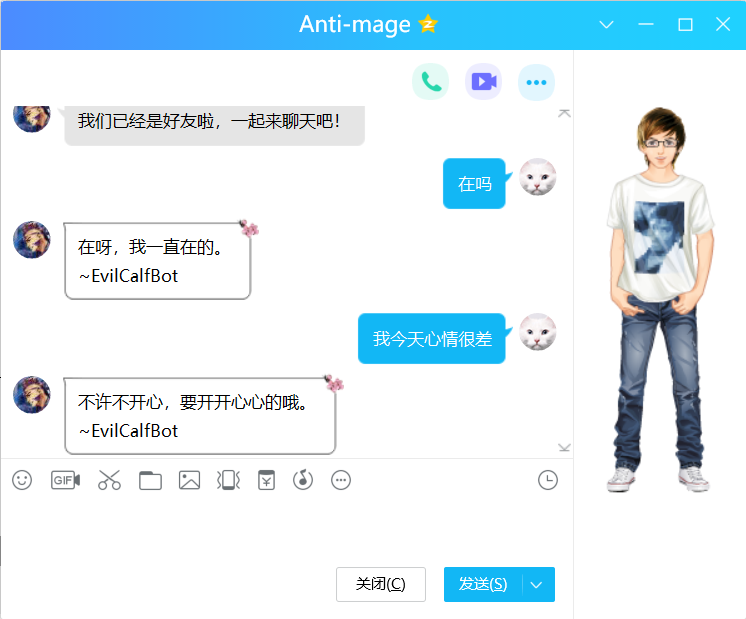
\includegraphics[width=\textwidth]{ECbot1}
      \caption{}
      \label{fig:ECbot1}
    \end{subfigure}%
    ~% add desired spacing
    \begin{subfigure}[b]{0.4\textwidth}
      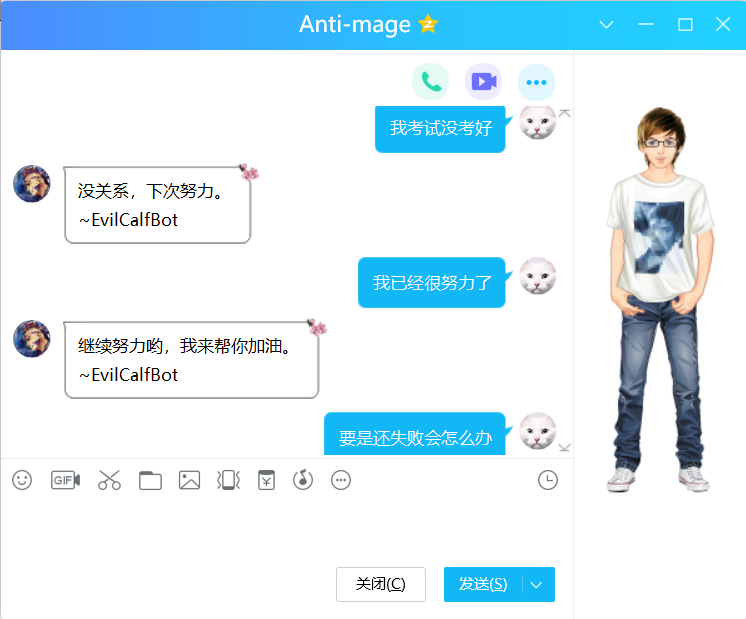
\includegraphics[width=\textwidth]{ECbot2}
      \caption{}
      \label{fig:ECbot2}
    \end{subfigure}
    \begin{subfigure}[b]{0.4\textwidth}
      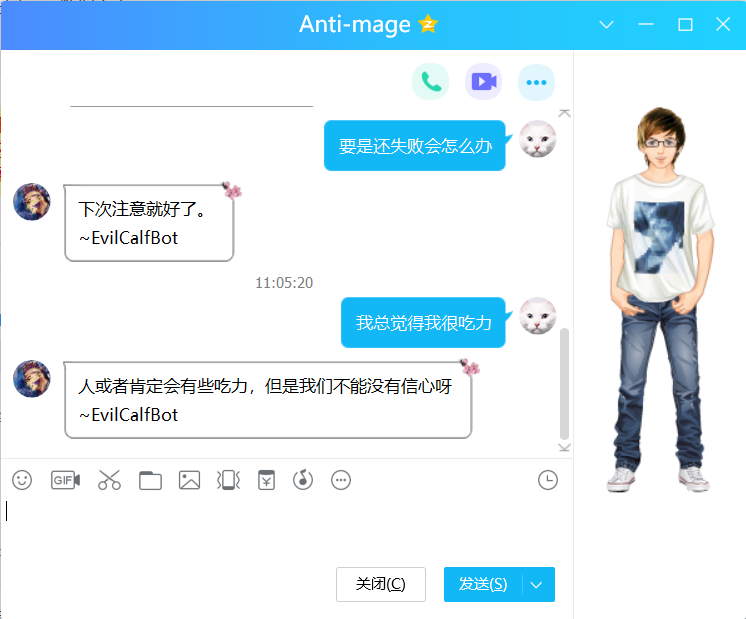
\includegraphics[width=\textwidth]{ECbot3}
      \caption{}
      \label{fig:ECbot3}
    \end{subfigure}%
    ~% add desired spacing
    \begin{subfigure}[b]{0.4\textwidth}
      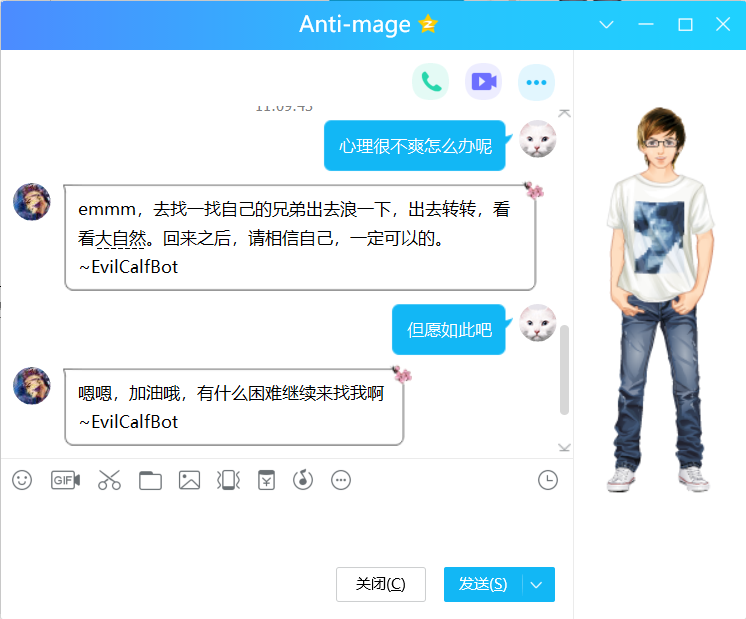
\includegraphics[width=\textwidth]{ECbot4}
      \caption{}
      \label{fig:ECbot4}
    \end{subfigure}
    \caption[总声压级]{实机测试图片}
    \label{fig:ECbot}
\end{figure}

嵌入常用的社交软件QQ之后,能几乎没有延迟的回复接受到的消息,这得益于UDP的高效的性能。自由的设置白名单可以对不同类型的好友进行区分,对于工作相关的好友,专业性重,突发性个性化也较强,对这些对话进行分析回复的效果同样不是非常优秀,可以设置关闭功能。而对于日常朋友的闲聊来说,可以及时的回复,无疑是大有帮助的。
\end{cuzchapter}
% Guidance
\begin{cuzchapter}{总结与未来工作}{chap:conclusions}
\section{总结}\label{sec:background}
使用序列到序列模型实现面向任务的对话模型,在日常闲聊的语料库上进行了端到端的培训,并与几个基线进行了比较。我们的模型可以在没有任何先前的领域知识的情况下学习语言以进行基本对话。

该模型最明显的问题是,当需要完全匹配使用正确的实体会遇到麻烦。该模型倾向于使用在训练期间看到的回复而不是使用来自上下文的实体。从未使用过训练期间未见过的单词,这意味着系统无法在没有再培训的情况下处理新实体。系统在这些关键任务上的失败会使其不适合用作独立的聊天机器人。然而,这些测试显示了在面向任务的对话环境中序列到序列模型的一些优点和局限性。这些知识可用于未来的测试和开发。

本论文的目的是学习以及实践研发聊天机器人,并对对话系统的各种模型进行测试分析。测试已实施系统的性能,其拥有很多优势,但也存在不容忽视的重大缺陷。

总之,我们目前的模型不能用作独立系统来成功进行完整对话,不能达到真正的人工智能。特别是中文的语言太博大精深,如果让机器学习并且理解,可能还需要更多的对分词标注技术进行提高。本论文对神经网络所训练出的模型进行一定的评估,并能显示出其在未来工作中可能发挥最大作用的地方,同时可以为未来的工作提供经验。
\section{未来工作}\label{sec:background}
本论文的工作仅限于一个相当小的领域。可能需要对其他可能更广泛的领域进行测试,以了解结果如何扩展。与本论文中讨论的模型相比,尝试其他学习模型并评估其性能也是有意义的。存在许多不同的基于神经网络的会话模型,每个会话模型都有自己的优点和缺点。

对序列到序列模型有一些可能的修改,这些修改对于聊天机器人的研发是有改进意义的。一种修改是尝试使用完全匹配,另一种修改是用更高级的算法(例如波束搜索)替换响应生成中的贪婪搜索。

本文的模型采取逐字生成响应。一种可能的改进是实现基于检索的响应生成。基于检索的推理功能应该能够提高准确性并允许更多地控制答案。因此,我们可以避免我们现在拥有的无意义和语法错误的句子。缺点是对可能的答案的限制以及创建答案集所需的额外努力,还存在增加的计算成本。

基于规则的模型在更简单的结构化任务上优于基于网络的模型,而基于网络的模型在更加非结构化的任务上表现更好。因此,制作结合两种方法的优势的混合模型将更有前途的。在某些情况下,我们真正需要的是匹配某个单词,但是如果我们从一开始就根据我们的领域知识制定规则,那么它将不存在端到端的可训练性和系统的可移植性。然而,这可能是当今实施聊天机器人系统的合理方法,因为当前的神经网络远不够准确,可能无法自行工作。

在聊天机器人的应用中,不仅仅是准确性很重要,用户在使用系统时的感受同样重要。由于本文的目的是评估使用神经网络创建聊天机器人的能力,因此应用程序几乎仅使用序列到序列模型而不是其他任何东西。因此,有许多改进可以带来增强的用户体验。一个简单的改进是计算在对话的每个步骤中我们的响应的概率,并且如果概率低于某个阈值则给用户以一种万金油的方式。必须适当设置此阈值,以使消息不会过于频繁地显示并产生额外的烦恼。有时聊天机器人的响应方式不会朝着用户想要的方向发展。当这个错误的响应进入上下文时,它可能会在进行未来预测时混淆聊天机器人。解决这个问题的方法可能是检测我们何时发生错误而不将该部分附加到上下文。

最后是因为中文的特点,本文的训练难度和英文比起来相差非常之大,同等文本下,中文的语料库训练出的维度会多很多,并且词向量之间的距离和关系的处理难度也更大。目前的NLP水平可能还不足以完美地对中文语言进行切词。也许我们需要更多的努力对中文NLP进行研究学习。

上面我们已经提到了一些基于本论文发现的想法,但是在这个研究领域的中,未来的工作还有更多的可能性等着我们去研究。
\end{cuzchapter}% Conclusions
%---------------------------------------------------------------------------%
%
%-
%-> Backmatter: acknowledgement, references, appendices (if any)
%-
%-> The acknowledgement
\begin{acknowledgement}
    感谢指导老师昊哥的付出!感谢身边的同学!感谢国内外各方大牛的论文!感谢其他学院有着同样兴趣爱好的同学们!感谢LaTex以及相关大学模板的制作者!感谢所有帮助过我的人!若无上述帮助与参考,我无法完成此论文的制作。大学四年的学习生活以本文作出的最后的总结,将其作为我踏入学术世界大门的第一次敲门。希望未来读研的日子里不会忘记了第一次书写论文的时的热情和激情,为学术事业奉献终身。当然此论文尚有许多不足之处,然可在后面不断完善。
    
    最后,再次对上述人士表示衷心感谢!
\end{acknowledgement}%
%-> The references
\intotoc{\bibname}% add link to contents table and bookmark
\begingroup
    \linespread{1.2}\selectfont
    \bibliography{bibliography/references}%
\endgroup
%-> The appendices (if any)
\appendix% change the page layout
% \chapter{中国科学院大学学位论文撰写要求}
\begin{appendices}\label{sec:appendices}
    \section*{附录代码段合集} \label{sec:testlistings}
    \begin{lstlisting}[
        language=python,
        label=code:catch,
        caption=自动抓取字幕
    ]
    # coding:utf-8
    import sys
    reload(sys)
    sys.setdefaultencoding( "utf-8" )
    
    import scrapy
    from w3lib.html import remove_tags
    from subtitle_crawler.items import SubtitleCrawlerItem
    
    class SubTitleSpider(scrapy.Spider):
        name = "subtitle"
        allowed_domains = ["zimuku.net"]
        start_urls = [
                "http://www.zimuku.net/search?q=&t=onlyst&ad=1&p=20",
                "http://www.zimuku.net/search?q=&t=onlyst&ad=1&p=21",
                "http://www.zimuku.net/search?q=&t=onlyst&ad=1&p=22",
        ]
    
        def parse(self, response):
            hrefs = response.selector.xpath('//div[contains(@class, "persub")]/h1/a/@href').extract()
            for href in hrefs:
                url = response.urljoin(href)
                request = scrapy.Request(url, callback=self.parse_detail)
                yield request
    
        def parse_detail(self, response):
            url = response.selector.xpath('//li[contains(@class, "dlsub")]/div/a/@href').extract()[0]
            print "processing: ", url
            request = scrapy.Request(url, callback=self.parse_file)
            yield request
    
        def parse_file(self, response):
            body = response.body
            item = SubtitleCrawlerItem()
            item['url'] = response.url
            item['body'] = body
            return item
    \end{lstlisting}
    \begin{lstlisting}[
        language=python,
        label=code:catchm,
        caption=主函数
    ]
    class SubtitleCrawlerPipeline(object):
        def process_item(self, item, spider):
            url = item['url']
            file_name = url.replace('/','_').replace(':','_')
            fp = open('result/'+file_name, 'w')
            fp.write(item['body'])
            fp.close()
            return item
    \end{lstlisting}
    \begin{lstlisting}[
        language=python,
        label=code:mv_ass,
        caption=取出扩展名为ass的文件
    ]
    import glob
    import os
    import fnmatch
    import shutil
    import sys
    
    
    def iterfindfiles(path, fnexp):
        for root, dirs, files in os.walk(path):
            for filename in fnmatch.filter(files, fnexp):
                yield os.path.join(root, filename)
    
    
    i=0
    for filename in iterfindfiles(r"./input/", "*.ass"):
        i=i+1
        newfilename = "ass/" + str(i) + "_" + os.path.basename(filename)
        print filename + " <===> " + newfilename
        shutil.move(filename, newfilename)
        #sys.exit(-1)
    
    \end{lstlisting}
    \begin{lstlisting}[
        language=python,
        label=code:mv_Irc,
        caption=取出扩展名为Irc的文件
    ]
    import glob
    import os
    import fnmatch
    import shutil
    import sys
    
    
    def iterfindfiles(path, fnexp):
        for root, dirs, files in os.walk(path):
            for filename in fnmatch.filter(files, fnexp):
                yield os.path.join(root, filename)
    
    
    i=0
    for filename in iterfindfiles(r"./input/", "*.LRC"):
        i=i+1
        newfilename = "lrc/" + str(i) + "_" + os.path.basename(filename)
        print filename + " <===> " + newfilename
        shutil.move(filename, newfilename)
        #sys.exit(-1)
    
    \end{lstlisting}
    \begin{lstlisting}[
        language=python,
        label=code:mv_smi,
        caption=取出扩展名为smi的文件
    ]
    import glob
    import os
    import fnmatch
    import shutil
    import sys
    
    
    def iterfindfiles(path, fnexp):
        for root, dirs, files in os.walk(path):
            for filename in fnmatch.filter(files, fnexp):
                yield os.path.join(root, filename)
    
    
    i=0
    for filename in iterfindfiles(r"./input/", "*.SMI"):
        i=i+1
        newfilename = "smi/" + str(i) + "_" + os.path.basename(filename)
        print filename + " <===> " + newfilename
        shutil.move(filename, newfilename)
        #sys.exit(-1)
    \end{lstlisting}
    \begin{lstlisting}[
        language=python,
        label=code:mv_srt,
        caption=取出扩展名为srt的文件
    ]
    import glob
    import os
    import fnmatch
    import shutil
    import sys
    
    
    def iterfindfiles(path, fnexp):
        for root, dirs, files in os.walk(path):
            for filename in fnmatch.filter(files, fnexp):
                yield os.path.join(root, filename)
    
    
    i=0
    for filename in iterfindfiles(r"./input/", "*.SRT"):
        i=i+1
        newfilename = "srt/" + str(i) + "_" + os.path.basename(filename)
        print filename + " <===> " + newfilename
        shutil.move(filename, newfilename)
        #sys.exit(-1)
    
    \end{lstlisting}
    \begin{lstlisting}[
        language=python,
        label=code:mv_ssa,
        caption=取出扩展名为ssa的文件
    ]
    import glob
    import os
    import fnmatch
    import shutil
    import sys
    
    
    def iterfindfiles(path, fnexp):
        for root, dirs, files in os.walk(path):
            for filename in fnmatch.filter(files, fnexp):
                yield os.path.join(root, filename)
    
    
    i=0
    for filename in iterfindfiles(r"./input/", "*.ssa"):
        i=i+1
        newfilename = "ssa/" + str(i) + "_" + os.path.basename(filename)
        print filename + " <===> " + newfilename
        shutil.move(filename, newfilename)
        #sys.exit(-1)
    
    \end{lstlisting}
    \begin{lstlisting}[
        language=python,
        label=code:mv_str,
        caption=取出扩展名为str的文件
    ]
    import glob
    import os
    import fnmatch
    import shutil
    import sys
    
    
    def iterfindfiles(path, fnexp):
        for root, dirs, files in os.walk(path):
            for filename in fnmatch.filter(files, fnexp):
                yield os.path.join(root, filename)
    
    
    i=0
    for filename in iterfindfiles(r"./input/", "*.str"):
        i=i+1
        newfilename = "str/" + str(i) + "_" + os.path.basename(filename)
        print filename + " <===> " + newfilename
        shutil.move(filename, newfilename)
        #sys.exit(-1)
    
    \end{lstlisting}
    \begin{lstlisting}[
        language=python,
        label=code:mv_sup,
        caption=取出扩展名为sup的文件
    ]
    import glob
    import os
    import fnmatch
    import shutil
    import sys
    
    
    def iterfindfiles(path, fnexp):
        for root, dirs, files in os.walk(path):
            for filename in fnmatch.filter(files, fnexp):
                yield os.path.join(root, filename)
    
    
    i=0
    for filename in iterfindfiles(r"./input/", "*.sup"):
        i=i+1
        newfilename = "sup/" + str(i) + "_" + os.path.basename(filename)
        print filename + " <===> " + newfilename
        shutil.move(filename, newfilename)
        #sys.exit(-1)
    
    \end{lstlisting}
    \begin{lstlisting}[
        language=python,
        label=code:mv_vtt,
        caption=取出扩展名为vtt的文件
    ]
    import glob
    import os
    import fnmatch
    import shutil
    import sys
    
    
    def iterfindfiles(path, fnexp):
        for root, dirs, files in os.walk(path):
            for filename in fnmatch.filter(files, fnexp):
                yield os.path.join(root, filename)
    
    
    i=0
    for filename in iterfindfiles(r"./input/", "*.vtt"):
        i=i+1
        newfilename = "vtt/" + str(i) + "_" + os.path.basename(filename)
        print filename + " <===> " + newfilename
        shutil.move(filename, newfilename)
        #sys.exit(-1)
    \end{lstlisting}
    \begin{lstlisting}[
        language=python,
        label=code:encode,
        caption=编码识别与转码
    ]
    import chardet
    import sys
    import os
    
    if __name__ == '__main__':
        if len(sys.argv) == 2:
            for root, dirs, files in os.walk(sys.argv[1]):
                for file in files:
                    file_path = root + "/" + file
                    f = open(file_path,'r')
                    data = f.read()
                    f.close()
                    encoding = chardet.detect(data)["encoding"]
                    if encoding not in ("UTF-8-SIG", "UTF-16LE", "utf-8", "ascii"):
                        try:
                            gb_content = data.decode("gb18030")
                            gb_content.encode('utf-8')
                            f = open(file_path, 'w')
                            f.write(gb_content.encode('utf-8'))
                            f.close()
                        except:
                            print "except:", file_path
    \end{lstlisting}
    \begin{lstlisting}[
        language=python,
        label=code:extract,
        caption=筛选中文
    ]
    # coding:utf-8
    import chardet
    import os
    import re
    
    cn=ur"([\u4e00-\u9fa5]+)"
    pattern_cn = re.compile(cn)
    jp1=ur"([\u3040-\u309F]+)"
    pattern_jp1 = re.compile(jp1)
    jp2=ur"([\u30A0-\u30FF]+)"
    pattern_jp2 = re.compile(jp2)
    
    for root, dirs, files in os.walk("./srt"):
        file_count = len(files)
        if file_count > 0:
            for index, file in enumerate(files):
                f = open(root + "/" + file, "r")
                content = f.read()
                f.close()
                encoding = chardet.detect(content)["encoding"]
                try:
                    for sentence in content.decode(encoding).split('\n'):
                        if len(sentence) > 0:
                            match_cn =  pattern_cn.findall(sentence)
                            match_jp1 =  pattern_jp1.findall(sentence)
                            match_jp2 =  pattern_jp2.findall(sentence)
                            sentence = sentence.strip()
                            if len(match_cn)>0 and len(match_jp1)==0 and len(match_jp2) == 0 and len(sentence)>1 and len(sentence.split(' ')) < 10:
                                print sentence.encode('utf-8')
                except:
                    continue
    \end{lstlisting}
    \begin{lstlisting}[
        language=python,
        label=code:filter,
        caption=内容过滤
    ]
    # coding:utf-8
    import sys
    import re
    import chardet
    
    if __name__ == '__main__':
        #illegal=r"([\u2000-\u2010]+)"
        illegal=r"([\u0000-\u2010]+)"
        pattern_illegals = [re.compile(r"([\u2000-\u2010]+)"), re.compile(r"([\u0090-\u0099]+)")]
        filters = ["字幕", "时间轴:", "校对:", "翻译:", "后期:", "监制:"]
        filters.append("时间轴:")
        filters.append("校对:")
        filters.append("翻译:")
        filters.append("后期:")
        filters.append("监制:")
        filters.append("禁止用作任何商业盈利行为")
        filters.append("http")
        htmltagregex = re.compile(r'<[^>]+>',re.S)
        brace_regex = re.compile(r'\{.*\}',re.S)
        slash_regex = re.compile(r'\\\w',re.S)
        repeat_regex = re.compile(r'[-=]{10}',re.S)
        f = open("./corpus/all.out", "r")
        count=0
        while True:
            line = f.readline()
            if line:
                line = line.strip()
    
                # 编码识别,不是utf-8就过滤
                gb_content = ''
                try:
                    gb_content = line.decode("utf-8")
                except Exception as e:
                    sys.stderr.write("decode error:  ", line)
                    continue
    
                # 中文识别,不是中文就过滤
                need_continue = False
                for pattern_illegal in pattern_illegals:
                    match_illegal = pattern_illegal.findall(gb_content)
                    if len(match_illegal) > 0:
                        sys.stderr.write("match_illegal error: %s\n" % line)
                        need_continue = True
                        break
                if need_continue:
                    continue
    
                # 关键词过滤
                need_continue = False
                for filter in filters:
                    try:
                        line.index(filter)
                        sys.stderr.write("filter keyword of %s %s\n" % (filter, line))
                        need_continue = True
                        break
                    except:
                        pass
                if need_continue:
                    continue
    
                # 去掉剧集信息
                if re.match('.*第.*季.*', line):
                    sys.stderr.write("filter copora %s\n" % line)
                    continue
                if re.match('.*第.*集.*', line):
                    sys.stderr.write("filter copora %s\n" % line)
                    continue
                if re.match('.*第.*帧.*', line):
                    sys.stderr.write("filter copora %s\n" % line)
                    continue
    
                # 去html标签
                line = htmltagregex.sub('',line)
    
                # 去花括号修饰
                line = brace_regex.sub('', line)
    
                # 去转义
                line = slash_regex.sub('', line)
    
                # 去重复
                new_line = repeat_regex.sub('', line)
                if len(new_line) != len(line):
                    continue
    
                # 去特殊字符
                line = line.replace('-', '').strip()
    
                if len(line) > 0:
                    sys.stdout.write("%s\n" % line)
                count+=1
            else:
                break
        f.close()
        pass
    
    \end{lstlisting}
    \begin{lstlisting}[
        language=java,
        label=code:inject,
        caption=页面注入
    ]
    public void injectQqSettingLayout() {
        XposedHelpers.findAndHookConstructor(QQSettingMe, classLoader,
                BaseActivity,
                QQAppInterface,
                FrameHelperActivity, new XC_MethodHook() {
                    @Override
                    protected void afterHookedMethod(MethodHookParam param) throws Throwable {
                        Field viewsField = XposedUtil.getField(param.thisObject, "a", View[].class);
                        if (viewsField != null) {
                            View[] views = (View []) viewsField.get(param.thisObject);
                            final LinearLayout linearLayout = (LinearLayout) views[0].getParent();
                            LayoutInflater layoutInflater = LayoutInflater.from(mContext);
                            LinearLayout injectLayout = (LinearLayout) layoutInflater.inflate(Setting_Layout_Id, null);
                            ((TextView)injectLayout.findViewById(Setting_TextView_Id)).setText("QQ机器人");
                            injectLayout.setOnClickListener(new View.OnClickListener() {
                                @Override
                                public void onClick(View v) {
                                    Intent intent = new Intent(Intent.ACTION_MAIN);
                                    intent.addCategory(Intent.CATEGORY_LAUNCHER);
                                    ComponentName cn = new ComponentName("cn.EvilCalf.ECBot", "cn.EvilCalf.ECBot.MainActivity");
                                    intent.setComponent(cn);
                                    linearLayout.getContext().startActivity(intent);
                                }
                            });
                            linearLayout.addView(injectLayout);
                        }
                    }
                });
    }
    \end{lstlisting}
    \begin{lstlisting}[
        language=java,
        label=code:socket,
        caption=SOCKET
    ]
    package cn.EvilCalf.ECBot;
    import java.io.IOException;
    import java.net.DatagramPacket;
    import java.net.DatagramSocket;
    import java.net.InetAddress;
    import java.net.SocketException;
    import java.net.UnknownHostException;
    
    public class socket
    {
        protected socket()
        {}
        public static void connectServerWithUDPSocket(String str) {
    
            DatagramSocket socket;
            try {
                socket = new DatagramSocket(1985);
                InetAddress serverAddress = InetAddress.getByName("120.78.197.104");
                byte data[] = str.getBytes();
                DatagramPacket packet = new DatagramPacket(data, data.length ,serverAddress ,10025);
                socket.send(packet);
            } catch (SocketException e) {
                e.printStackTrace();
            } catch (UnknownHostException e) {
                e.printStackTrace();
            } catch (IOException e) {
                e.printStackTrace();
            }
        }
        public static String ReceiveServerSocketData() {
            DatagramSocket socket;
            String result = null;
            try {
                socket = new DatagramSocket(1985);
                byte data[] = new byte[4 * 1024];
                DatagramPacket packet = new DatagramPacket(data, data.length);
                socket.receive(packet);
                result = new String(packet.getData(), packet.getOffset(),
                        packet.getLength());
                socket.close();
            } catch (SocketException e) {
                e.printStackTrace();
            } catch (IOException e) {
                e.printStackTrace();
            }
            return result;
        }
    }
    
    \end{lstlisting}
    \begin{lstlisting}[
        language=java,
        label=code:commnucation,
        caption=消息交互
    ]
    package cn.EvilCalf.ECBot.xposed;

    import android.content.Context;
    
    import com.zhy.http.okhttp.callback.StringCallback;
    
    import java.util.ArrayList;
    import java.util.Map;
    
    import cn.EvilCalf.ECBot.robot.Robot;
    import cn.EvilCalf.ECBot.xposed.utils.XLogUtil;
    import cn.EvilCalf.ECBot.xposed.utils.XPreferenceUtil;
    import cn.EvilCalf.ECBot.xposed.utils.XposedUtil;
    import de.robv.android.xposed.XC_MethodHook;
    import de.robv.android.xposed.XposedHelpers;
    import okhttp3.Call;
    
    import static cn.EvilCalf.ECBot.Common.BaseApplicationImpl;
    import static cn.EvilCalf.ECBot.Common.ChatActivityFacade;
    import static cn.EvilCalf.ECBot.Common.MessageHandlerUtils;
    import static cn.EvilCalf.ECBot.Common.MessageRecord;
    import static cn.EvilCalf.ECBot.Common.QQAppInterface;
    import static cn.EvilCalf.ECBot.Common.SendMsgParams;
    import static cn.EvilCalf.ECBot.Common.SessionInfo;
    import static cn.EvilCalf.ECBot.xposed.utils.XPreferenceUtil.getApiKey;
    import static cn.EvilCalf.ECBot.xposed.utils.XPreferenceUtil.getKeyReply;
    import static de.robv.android.xposed.XposedHelpers.callMethod;
    import static de.robv.android.xposed.XposedHelpers.callStaticMethod;
    import static de.robv.android.xposed.XposedHelpers.findAndHookMethod;
    import static de.robv.android.xposed.XposedHelpers.findClass;
    import static de.robv.android.xposed.XposedHelpers.getObjectField;
    import static de.robv.android.xposed.XposedHelpers.newInstance;
    
    
    
    public class MessageUtil extends BaseHook {
    
        private Object sApplication;
        private Context mContext;
    
        private MessageUtil(ClassLoader classLoader) {
            super(classLoader);
    
        }
    
        MessageUtil(ClassLoader classLoader, Context context) {
            super(classLoader);
            mContext = context;
        }
    
        public void initAutoReply() {
            sApplication = callStaticMethod(findClass(BaseApplicationImpl, classLoader), "getApplication");
            findAndHookMethod(MessageHandlerUtils, classLoader, "a",
                    QQAppInterface,
                    MessageRecord,
                    boolean.class, new XC_MethodHook() {
                        @Override
                        protected void afterHookedMethod(MethodHookParam param) throws Throwable {
                            XLogUtil.d("总开关", XPreferenceUtil.getMasterSwitch() + "");
                            if (!XPreferenceUtil.getMasterSwitch()) return;
    
                            final String frienduin = getObjectField(param.args[1], "frienduin").toString();
                            final String selfuin = getObjectField(param.args[1], "selfuin").toString();
                            final int istroop = (int) getObjectField(param.args[1], "istroop");
                            final String senderuin = getObjectField(param.args[1], "senderuin").toString();
                            final String msg = getObjectField(param.args[1], "msg").toString();
                            boolean isread = (boolean) getObjectField(param.args[1], "isread");
    
                            XLogUtil.d("frienduin", frienduin);
                            XLogUtil.d("selfuin", selfuin);
                            XLogUtil.d("senderuin", senderuin);
    
                            String[] whiteList = XPreferenceUtil.getWhiteList();
    
                            if (whiteList.length != 0 && !senderuin.equals(selfuin)) {
                                if (XPreferenceUtil.getNoReplyTroop() && istroop == 1) return;
                                iteratorWhiteList(frienduin, selfuin, msg, senderuin, istroop, isread, whiteList);
                            }
                        }
                    });
        }
    
        private void iteratorWhiteList(String frienduin, String selfuin, String msg, String senderuin, int istroop, boolean isread, String[] list) {
            for (String s : list) {
                if (frienduin.equals(s) && !isread && !frienduin.equals(selfuin)) {
                    XLogUtil.d("MessageUtil", "iteratorWhiteList is running...");
                    ArrayList<Map<String, String>> keyReply = getKeyReply();
                    if (keyReply != null && keyReply.size() != 0) {
                        for (Map<String, String> stringMap: keyReply){
                            if (stringMap.get("content").trim().equals(msg)) {
                                send(frienduin, selfuin, istroop, stringMap.get("reply_content"));
                                return;
                            }
                        }
                    }
                    Robot robot = new Robot(Robot.RobotType.TULING);
                    robot.setCallback(new ReplyCallback(frienduin, selfuin, istroop));
                    robot.init(getApiKey(), msg, senderuin);
                }
            }
        }
    
        private void send(String frienduin, String selfuin, int istroop, String s) {
            Object qqAppInterface = callMethod(sApplication, "getAppRuntime", selfuin);
            Object sessionInfo = newInstance(findClass(SessionInfo, classLoader));
            Object sendMsgParams = newInstance(findClass(SendMsgParams, classLoader));
            XposedUtil.setField(sessionInfo, "a", frienduin, String.class);
            XposedUtil.setField(sessionInfo, "a", istroop, int.class);
            callStaticMethod(XposedHelpers.findClass(ChatActivityFacade, classLoader), "a", qqAppInterface, mContext, sessionInfo, s, new ArrayList<>(), sendMsgParams);
        }
    
        private class ReplyCallback extends StringCallback {
    
            private String frienduin;
            private String selfuin;
            private int istroop;
    
            ReplyCallback(String frienduin, String selfuin, int istroop) {
                this.frienduin = frienduin;
                this.selfuin = selfuin;
                this.istroop = istroop;
            }
            @Override
            public void onError(Call call, Exception e, int id) {
    
            }
    
            @Override
            public void onResponse(String response, int id) {
                send(frienduin, selfuin, istroop, Robot.tulingReply(response));
            }
        }
    }
    
    \end{lstlisting}
    \begin{lstlisting}[
        language=python,
        label=code:word2rec,
        caption=分词并转化为词向量
    ]
    # coding:utf-8
import sys
import jieba


class WordToken(object):
    def __init__(self):
        self.START_ID = 4
        self.word2id_dict = {}
        self.id2word_dict = {}

    def load_file_list(self, file_list):
        global index
        words_count = {}
        for file in file_list:
            with open(file, 'r', encoding='UTF-8') as file_object:
                for line in file_object.readlines():
                    line = line.strip()
                    seg_list = jieba.cut(line)
                    for str in seg_list:
                        if str in words_count:
                            words_count[str] = words_count[str] + 1
                        else:
                            words_count[str] = 1

        sorted_list = [[v[1], v[0]] for v in words_count.items()]
        sorted_list.sort(reverse=True)
        for index, item in enumerate(sorted_list):
            word = item[1]
            self.word2id_dict[word] = self.START_ID + index
            self.id2word_dict[self.START_ID + index] = word
        return index

    def word2id(self, word):
        if not isinstance(word, str):
            print("Exception: error word not unicode")
            sys.exit(1)
        if word in self.word2id_dict:
            return self.word2id_dict[word]
        else:
            return None

    def id2word(self, i_d):
        i_d = int(i_d)
        if i_d in self.id2word_dict:
            return self.id2word_dict[i_d]
        else:
            return None

    \end{lstlisting}
    \begin{lstlisting}[
        language=java,
        label=code:inject,
        caption=页面注入
    ]
    public void injectQqSettingLayout() {
        XposedHelpers.findAndHookConstructor(QQSettingMe, classLoader,
                BaseActivity,
                QQAppInterface,
                FrameHelperActivity, new XC_MethodHook() {
                    @Override
                    protected void afterHookedMethod(MethodHookParam param) throws Throwable {
                        Field viewsField = XposedUtil.getField(param.thisObject, "a", View[].class);
                        if (viewsField != null) {
                            View[] views = (View []) viewsField.get(param.thisObject);
                            final LinearLayout linearLayout = (LinearLayout) views[0].getParent();
                            LayoutInflater layoutInflater = LayoutInflater.from(mContext);
                            LinearLayout injectLayout = (LinearLayout) layoutInflater.inflate(Setting_Layout_Id, null);
                            ((TextView)injectLayout.findViewById(Setting_TextView_Id)).setText("QQ机器人");
                            injectLayout.setOnClickListener(new View.OnClickListener() {
                                @Override
                                public void onClick(View v) {
                                    Intent intent = new Intent(Intent.ACTION_MAIN);
                                    intent.addCategory(Intent.CATEGORY_LAUNCHER);
                                    ComponentName cn = new ComponentName("cn.EvilCalf.ECBot", "cn.EvilCalf.ECBot.MainActivity");
                                    intent.setComponent(cn);
                                    linearLayout.getContext().startActivity(intent);
                                }
                            });
                            linearLayout.addView(injectLayout);
                        }
                    }
                });
    }
    \end{lstlisting}
    \begin{lstlisting}[
        language=java,
        label=code:get,
        caption=获取域
    ]
    public static Object getObjectField(Object obj, String fieldName) {
		try {
			return findField(obj.getClass(), fieldName).get(obj);
		} catch (IllegalAccessException e) {
			// should not happen
			XposedBridge.log(e);
			throw new IllegalAccessError(e.getMessage());
		} catch (IllegalArgumentException e) {
			throw e;
		}
    }
    public static Field findField(Class<?> clazz, String fieldName) {
		String fullFieldName = clazz.getName() + '#' + fieldName;

		if (fieldCache.containsKey(fullFieldName)) {
			Field field = fieldCache.get(fullFieldName);
			if (field == null)
				throw new NoSuchFieldError(fullFieldName);
			return field;
		}

		try {
			Field field = findFieldRecursiveImpl(clazz, fieldName);
			field.setAccessible(true);
			fieldCache.put(fullFieldName, field);
			return field;
		} catch (NoSuchFieldException e) {
			fieldCache.put(fullFieldName, null);
			throw new NoSuchFieldError(fullFieldName);
		}
	}
    public static Field getField(Object object, String fieldName, Type type) {
        Field[] fields = object.getClass().getDeclaredFields();
        for (Field field : fields) {
            if (field.getType() == type && field.getName().equals(fieldName)) {
                field.setAccessible(true);
                return field;
            }
        }
        return null;
    }
    \end{lstlisting}
\begin{lstlisting}[
    language=java,
    label=code:train,
    caption=训练模型
]
# coding:utf-8
import numpy as np
import tensorflow as tf
from tensorflow.contrib.legacy_seq2seq.python.ops import seq2seq
import word_token
import jieba
import win_unicode_console

win_unicode_console.enable()

input_seq_len = 5
output_seq_len = 5
PAD_ID = 0
GO_ID = 1
EOS_ID = 2
size = 8
init_learning_rate = 1
wordToken = word_token.WordToken()
max_token_id = wordToken.load_file_list(['question', 'answer'])
num_encoder_symbols = max_token_id + 5
num_decoder_symbols = max_token_id + 5


def get_id_list_from(sentence):
    sentence_id_list = []
    seg_list = jieba.cut(sentence)
    for str in seg_list:
        id = wordToken.word2id(str)
        if id:
            sentence_id_list.append(wordToken.word2id(str))
    return sentence_id_list


def get_train_set():
    global num_encoder_symbols, num_decoder_symbols
    train_set = []
    with open('question', 'r', encoding='UTF-8') as question_file:
        with open('answer', 'r', encoding='UTF-8') as answer_file:
            while True:
                question = question_file.readline()
                answer = answer_file.readline()
                if question and answer:
                    question = question.strip()
                    answer = answer.strip()

                    question_id_list = get_id_list_from(question)
                    answer_id_list = get_id_list_from(answer)
                    answer_id_list.append(EOS_ID)
                    train_set.append([question_id_list, answer_id_list])
                else:
                    break
    return train_set


def get_samples(train_set):
    raw_encoder_input = []
    raw_decoder_input = []
    for sample in train_set:
        raw_encoder_input.append([PAD_ID] * (input_seq_len - len(sample[0])) + sample[0])
        raw_decoder_input.append([GO_ID] + sample[1] + [PAD_ID] * (output_seq_len - len(sample[1]) - 1))

    encoder_inputs = []
    decoder_inputs = []
    target_weights = []

    for length_idx in range(input_seq_len):
        encoder_inputs.append(
            np.array([encoder_input[length_idx] for encoder_input in raw_encoder_input], dtype=np.int32))
    for length_idx in range(output_seq_len):
        decoder_inputs.append(
            np.array([decoder_input[length_idx] for decoder_input in raw_decoder_input], dtype=np.int32))
        target_weights.append(np.array([
            0.0 if length_idx == output_seq_len - 1 or decoder_input[length_idx] == PAD_ID else 1.0 for decoder_input in
            raw_decoder_input
        ], dtype=np.float32))
    return encoder_inputs, decoder_inputs, target_weights


def get_model(feed_previous=False):
    learning_rate = tf.Variable(float(init_learning_rate), trainable=False, dtype=tf.float32)
    learning_rate_decay_op = learning_rate.assign(learning_rate * 0.9)

    encoder_inputs = []
    decoder_inputs = []
    target_weights = []
    for i in range(input_seq_len):
        encoder_inputs.append(tf.placeholder(tf.int32, shape=[None], name="encoder{0}".format(i)))
    for i in range(output_seq_len + 1):
        decoder_inputs.append(tf.placeholder(tf.int32, shape=[None], name="decoder{0}".format(i)))
    for i in range(output_seq_len):
        target_weights.append(tf.placeholder(tf.float32, shape=[None], name="weight{0}".format(i)))

    targets = [decoder_inputs[i + 1] for i in range(output_seq_len)]

    cell = tf.contrib.rnn.BasicLSTMCell(size)

    outputs, _ = seq2seq.embedding_attention_seq2seq(
        encoder_inputs,
        decoder_inputs[:output_seq_len],
        cell,
        num_encoder_symbols=num_encoder_symbols,
        num_decoder_symbols=num_decoder_symbols,
        embedding_size=size,
        output_projection=None,
        feed_previous=feed_previous,
        dtype=tf.float32)

    loss = seq2seq.sequence_loss(outputs, targets, target_weights)
    opt = tf.train.GradientDescentOptimizer(learning_rate)
    update = opt.apply_gradients(opt.compute_gradients(loss))
    saver = tf.train.Saver(tf.global_variables())

    return encoder_inputs, decoder_inputs, target_weights, outputs, loss, update, saver, learning_rate_decay_op, learning_rate


def train():
    train_set = get_train_set()
    with tf.Session() as sess:

        sample_encoder_inputs, sample_decoder_inputs, sample_target_weights = get_samples(train_set)
        encoder_inputs, decoder_inputs, target_weights, outputs, loss, update, saver, learning_rate_decay_op, learning_rate = get_model()

        input_feed = {}
        for l in range(input_seq_len):
            input_feed[encoder_inputs[l].name] = sample_encoder_inputs[l]
        for l in range(output_seq_len):
            input_feed[decoder_inputs[l].name] = sample_decoder_inputs[l]
            input_feed[target_weights[l].name] = sample_target_weights[l]
        input_feed[decoder_inputs[output_seq_len].name] = np.zeros([len(sample_decoder_inputs[0])], dtype=np.int32)

        sess.run(tf.global_variables_initializer())

        previous_losses = []
        for step in range(20700):
            [loss_ret, _] = sess.run([loss, update], input_feed)
            if step % 10 == 0:
                print('step=', step, 'loss=', loss_ret, 'learning_rate=', learning_rate.eval())

                if len(previous_losses) > 5 and loss_ret > max(previous_losses[-5:]):
                    sess.run(learning_rate_decay_op)
                previous_losses.append(loss_ret)

                saver.save(sess, './model/EvilCalf')


if __name__ == "__main__":
    train()

\end{lstlisting}
\begin{lstlisting}[
    language=java,
    label=code:predict,
    caption=预测模型
]
# coding:utf-8
import sys
import numpy as np
import tensorflow as tf
from tensorflow.contrib.legacy_seq2seq.python.ops import seq2seq
import word_token
import jieba
import win_unicode_console

win_unicode_console.enable()

input_seq_len = 5
output_seq_len = 5
PAD_ID = 0
GO_ID = 1
EOS_ID = 2
size = 8
init_learning_rate = 1
wordToken = word_token.WordToken()
max_token_id = wordToken.load_file_list(['question', 'answer'])
num_encoder_symbols = max_token_id + 5
num_decoder_symbols = max_token_id + 5


def get_id_list_from(sentence):
    sentence_id_list = []
    seg_list = jieba.cut(sentence)
    for str in seg_list:
        id = wordToken.word2id(str)
        if id:
            sentence_id_list.append(wordToken.word2id(str))
    return sentence_id_list


def seq_to_encoder(input_seq):
    input_seq_array = [int(v) for v in input_seq.split()]
    encoder_input = [PAD_ID] * (input_seq_len - len(input_seq_array)) + input_seq_array
    decoder_input = [GO_ID] + [PAD_ID] * (output_seq_len - 1)
    encoder_inputs = [np.array([v], dtype=np.int32) for v in encoder_input]
    decoder_inputs = [np.array([v], dtype=np.int32) for v in decoder_input]
    target_weights = [np.array([1.0], dtype=np.float32)] * output_seq_len
    return encoder_inputs, decoder_inputs, target_weights


def get_model(feed_previous=False):
    learning_rate = tf.Variable(float(init_learning_rate), trainable=False, dtype=tf.float32)
    learning_rate_decay_op = learning_rate.assign(learning_rate * 0.9)

    encoder_inputs = []
    decoder_inputs = []
    target_weights = []
    for i in range(input_seq_len):
        encoder_inputs.append(tf.placeholder(tf.int32, shape=[None], name="encoder{0}".format(i)))
    for i in range(output_seq_len + 1):
        decoder_inputs.append(tf.placeholder(tf.int32, shape=[None], name="decoder{0}".format(i)))
    for i in range(output_seq_len):
        target_weights.append(tf.placeholder(tf.float32, shape=[None], name="weight{0}".format(i)))

    targets = [decoder_inputs[i + 1] for i in range(output_seq_len)]

    cell = tf.contrib.rnn.BasicLSTMCell(size)

    outputs, _ = seq2seq.embedding_attention_seq2seq(
        encoder_inputs,
        decoder_inputs[:output_seq_len],
        cell,
        num_encoder_symbols=num_encoder_symbols,
        num_decoder_symbols=num_decoder_symbols,
        embedding_size=size,
        output_projection=None,
        feed_previous=feed_previous,
        dtype=tf.float32)

    loss = seq2seq.sequence_loss(outputs, targets, target_weights)
    opt = tf.train.GradientDescentOptimizer(learning_rate)
    update = opt.apply_gradients(opt.compute_gradients(loss))
    saver = tf.train.Saver(tf.global_variables())

    return encoder_inputs, decoder_inputs, target_weights, outputs, loss, update, saver, learning_rate_decay_op, learning_rate


def predict():
    with tf.Session() as sess:
        encoder_inputs, decoder_inputs, target_weights, outputs, loss, update, saver, learning_rate_decay_op, learning_rate = get_model(
            feed_previous=True)
        saver.restore(sess, './model/EvilCalf')
        sys.stdout.write("> ")
        sys.stdout.flush()
        input_seq = sys.stdin.readline()
        while input_seq:
            input_seq = input_seq.strip()
            input_id_list = get_id_list_from(input_seq)
            if len(input_id_list):
                sample_encoder_inputs, sample_decoder_inputs, sample_target_weights = seq_to_encoder(
                    ' '.join([str(v) for v in input_id_list]))

                input_feed = {}
                for l in range(input_seq_len):
                    input_feed[encoder_inputs[l].name] = sample_encoder_inputs[l]
                for l in range(output_seq_len):
                    input_feed[decoder_inputs[l].name] = sample_decoder_inputs[l]
                    input_feed[target_weights[l].name] = sample_target_weights[l]
                input_feed[decoder_inputs[output_seq_len].name] = np.zeros([2], dtype=np.int32)

                outputs_seq = sess.run(outputs, input_feed)
                outputs_seq = [int(np.argmax(logit[0], axis=0)) for logit in outputs_seq]
                if EOS_ID in outputs_seq:
                    outputs_seq = outputs_seq[:outputs_seq.index(EOS_ID)]
                outputs_seq = [wordToken.id2word(v) for v in outputs_seq]
                print(" ".join(outputs_seq))
            else:
                print("换句话吧,这句话无解,GG")

            sys.stdout.write("> ")
            sys.stdout.flush()
            input_seq = sys.stdin.readline()


if __name__ == "__main__":
    predict()

\end{lstlisting}
\end{appendices}%
\end{document}
%---------------------------------------------------------------------------%

